% Chapter 3

\chapter{Sensitivity study} % Main chapter title

\label{Chapter3} % For referencing the chapter elsewhere, use \ref{Chapter1} 

\lhead{3. \emph{Sensitivity Study}} % This is for the header on each page - perhaps a shortened title

\section{Synthetic Data}

Testing the performance of a model is a crucial step in defining new ground motion relationships and should always accompany the process of creating models. Especially in seismic risk evaluation one is interested how different parameters influence the reliability of the result. A sensitivity study evaluates the performance and gives the user a guide how to use a model in real life applications, how to quantify possible errors and which parameter should be given a higher priority in order to minimize uncertainties efficiently.
To test the performance of the model from \cite{Rotondi2004} first, a series of tests is performed on a set of synthetic intensity data. The synthetic data is constructed by sampling 700 distance values uniformly over a range of 300 kilometres. In order to calculate corresponding intensity values the model of \cite{Koveslighety1906} is used together with an epicentral intensity($I_0$) of IX:
\vspace{0.1cm}
\begin{equation}
\Delta I = a * log_{10}\left(\dfrac{d_h}{h}\right) + a * b * log(d_h -h)
\label{eqn:koveslighety}
\end{equation}

\begin{figure}[!htpb]
	\centering
		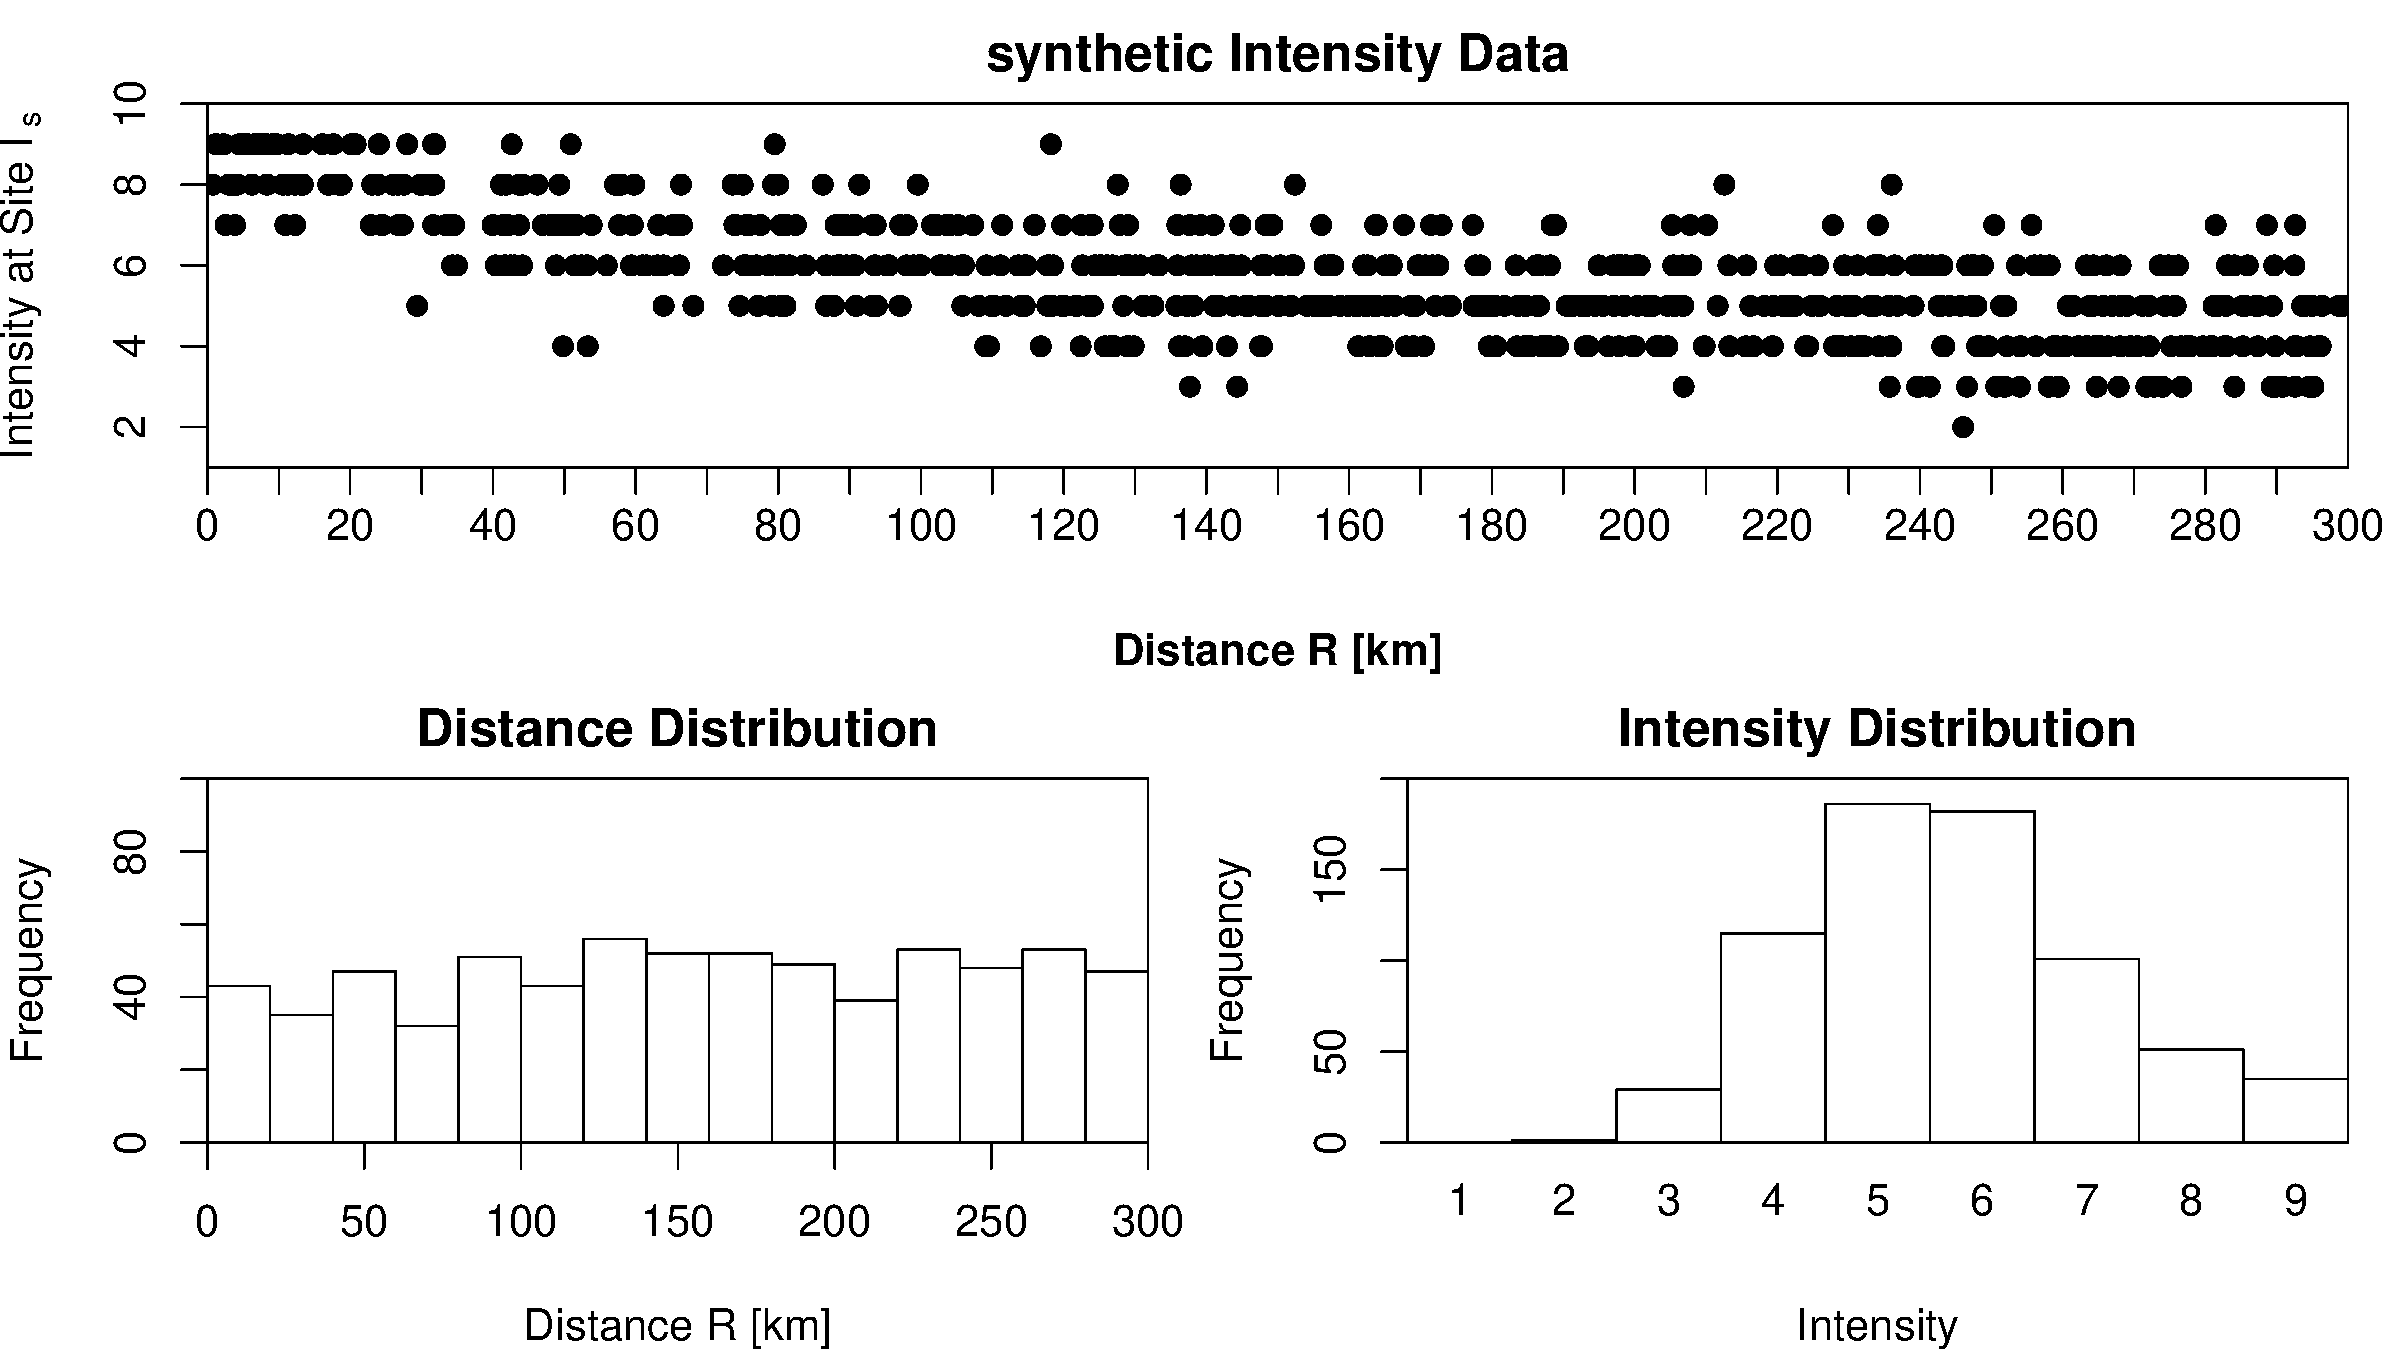
\includegraphics[scale=0.33]{Figures/dataDistro.pdf}
		\rule{35em}{0.5pt}
	\caption[synthetic data]{Synthetic data according to equation \ref{eqn:koveslighety}. Distance values where uniformly sampled over a distance range up to 300 kilometers.}
	\label{fig:dataDistro}
\end{figure}

where
$d_h = \sqrt{R^2+h^2}$ is the hypocentral distance of the earthquake, h = 10km is the depth of the earthquake hypocentre, $a$ = 3 is a factor for the geometrical spreading of seismic waves and $b = 0.002 km^{-1}$ is a parameter that accounts for the anelastic dissipation \citep{stromeyer2009attenuation}. To attain whole numbers the results of equation \ref{eqn:koveslighety} are rounded. As prior distribution a uniform distribution over the range between 0 and 1 is used corresponding to the hyperparameters of the Beta distribution $\alpha = \beta = 1$.



To estimate the prediction performance the mode of the binomial distribution for each distance bin is used in order to forecast intensities. The mean absolute error between predicted and synthetic intensities is the measure for the prediction ability.

\section{Data Size}

One important and very limiting factor for generating new ground motion models is the amount of data that is available. Depending on the region one might encounter scenarios where rich catalogues of past seismicity are available or just a sparse set of observations. To test the behaviour of the model in these different environments the synthetic data has been randomly partitioned into subsets of stepwise increasing number of observation, thus simulating the effect of different catalogue sizes. To estimate the model's performance a 10-fold cross-validation procedure is adopted to estimate the training error (in-sample error) as a measure of how well the model can approximate the data and the cross-validation error (out-of-sample error) which examines the performance on data that was not used in estimating the parameters of the model. Also it is a very easy way to qualitatively diagnose whether the model is suffering from bias or variance. Bias means the model's ability to approximate the target function that has generated the data. Variance quantifies how sensitive this estimate is to a specific subset of the data.  In a high bias case fit and cross-validation error would rapidly approach each other and remain equal on a high level. This means that adding more data does not improve the models performance since the model that is used to fit the target function can only approximate it poorly. It is a case of underfitting. Conversely, in a high variance scenario there is a gap between fit and cross-validation error but the cross-validation error still decreases with more data. This situation corresponds to overfitting.\\
 
\begin{figure}[!htpb]
	\centering
		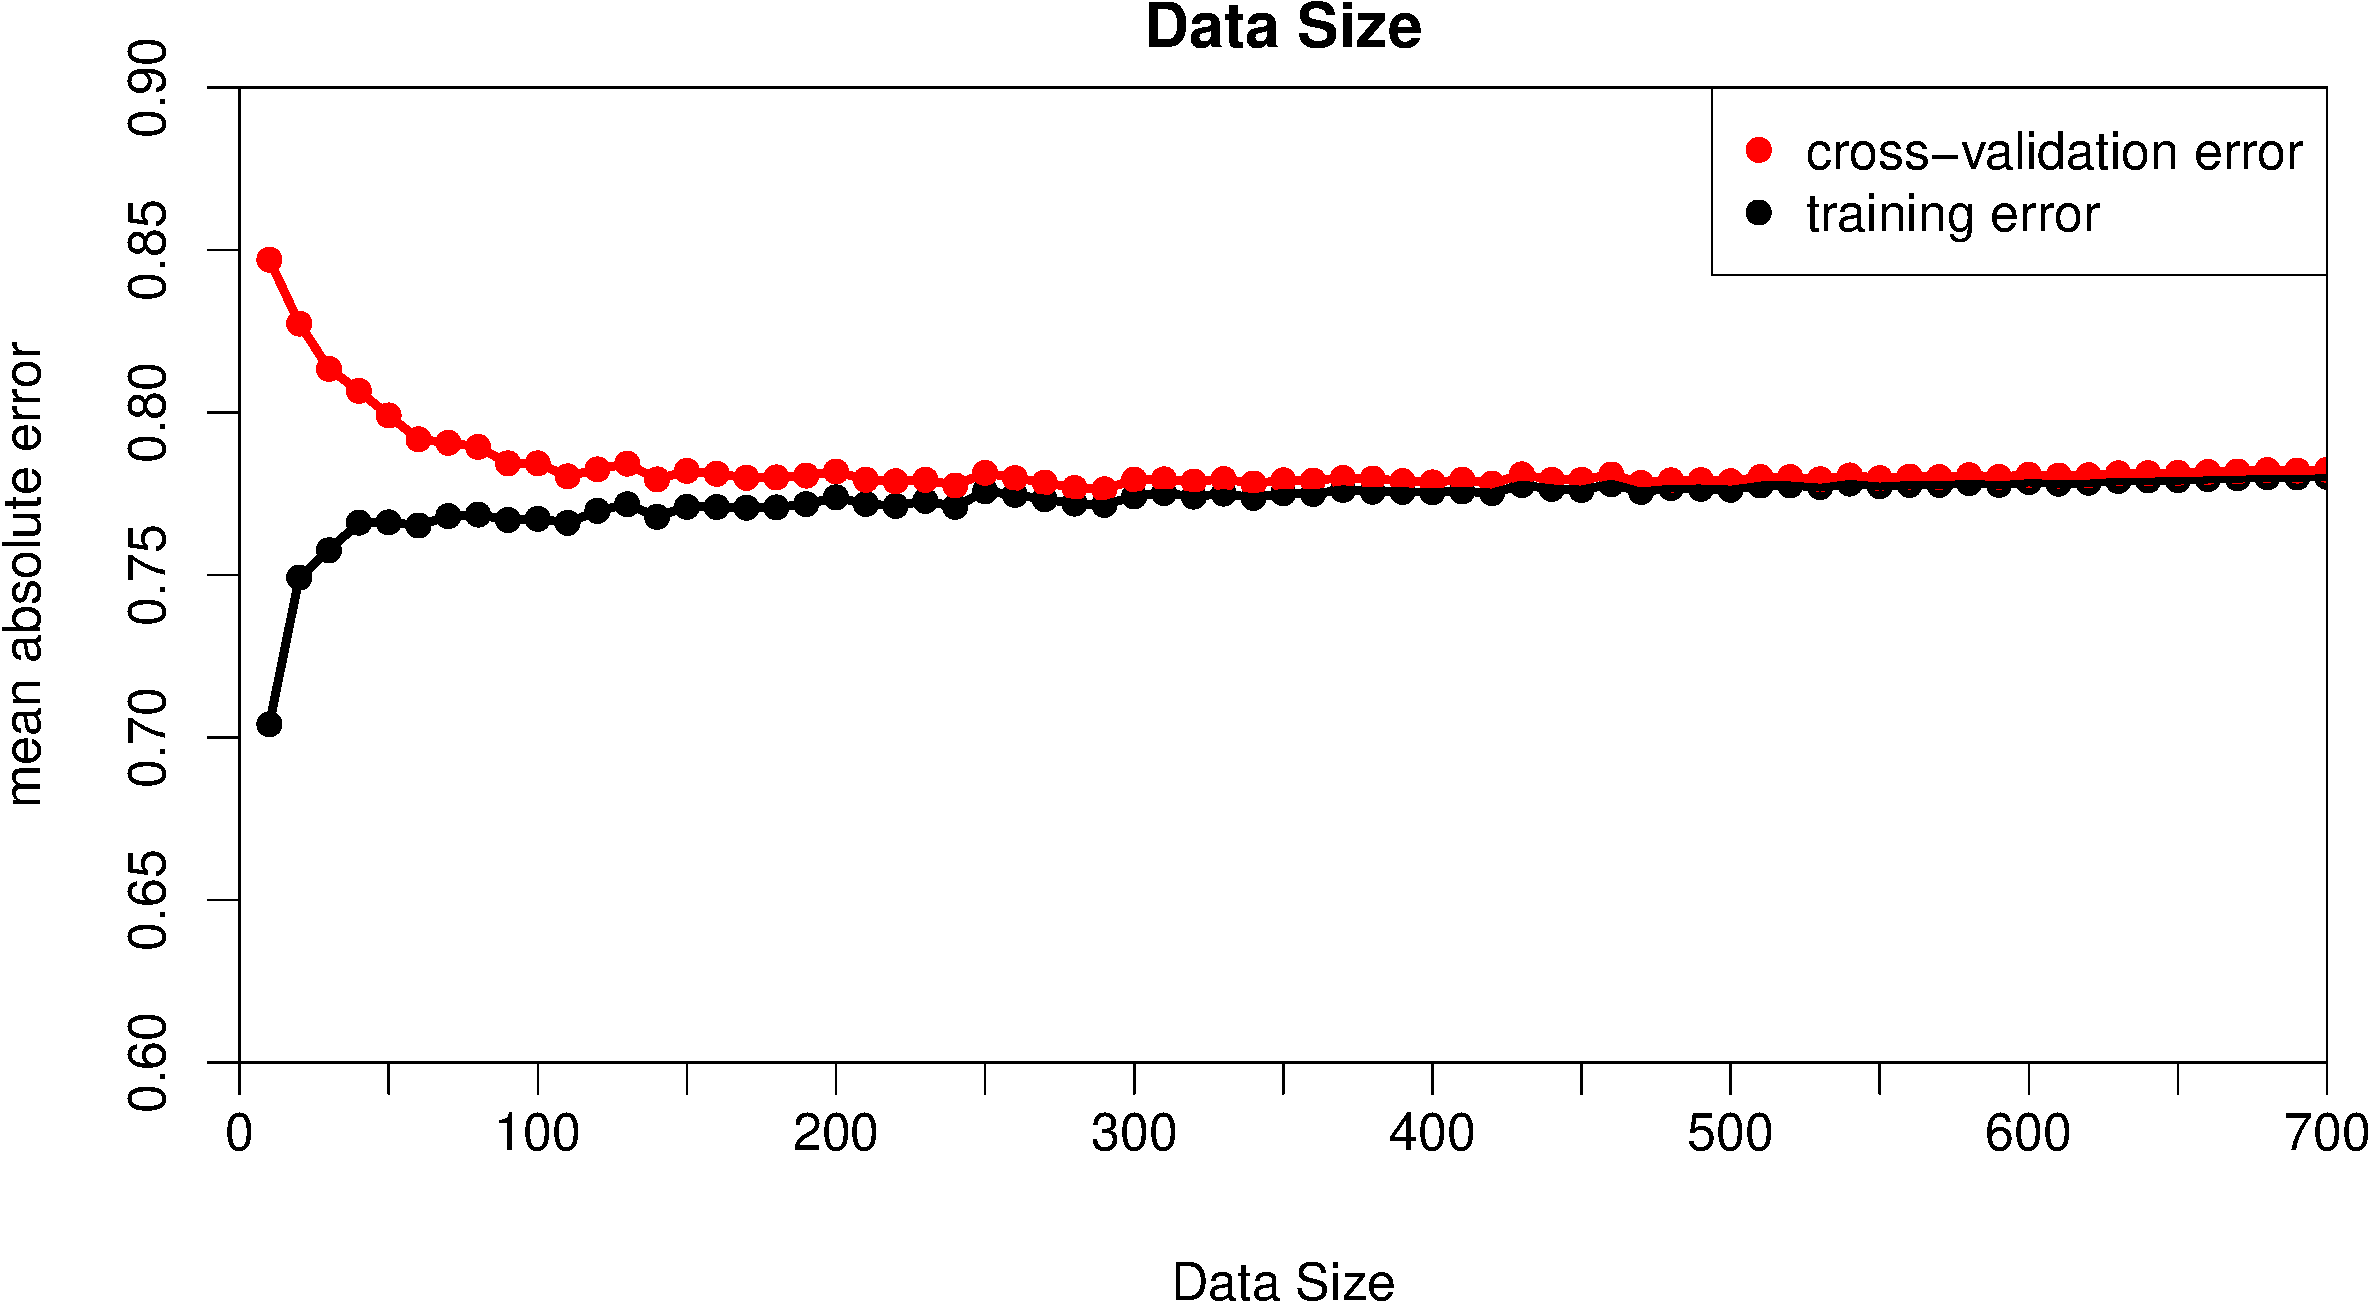
\includegraphics[scale=0.33]{Figures/numberData.pdf}
		\rule{35em}{0.5pt}
	\caption[Data Size]{Data Size}
	\label{fig:data}
\end{figure}

Figure \ref{fig:data} shows the results of this analysis. With a small data set size the cross-validation error is larger than the training error. This means that the trained model does not well generalize to unseen data. Increasing the data set size results in decreasing cross-validation error and increasing training error. Though it becomes harder to replicate all of the training data the model performs better in predicting. At around 500 data samples there is no real difference between cross-validation and training error. 

\section{Quality of the Data}
Another parameter that can heavily influence the computation of new ground motion relationships is the quality of the data. The best algorithm can only perform as well as the used data. To simulate the effect of poor data a Gaussian error with a mean equal to zero and a stepwise increasing standard deviation is added to synthetic data. Since only the isolated effect of poor data should be studied the whole 1000 synthetic observations are used. Because at this data size there is no difference in training error and cross-validation error only the cross-validation error is shown in Figure \ref{fig:noise}.

\begin{figure}[!htb]
	\centering
		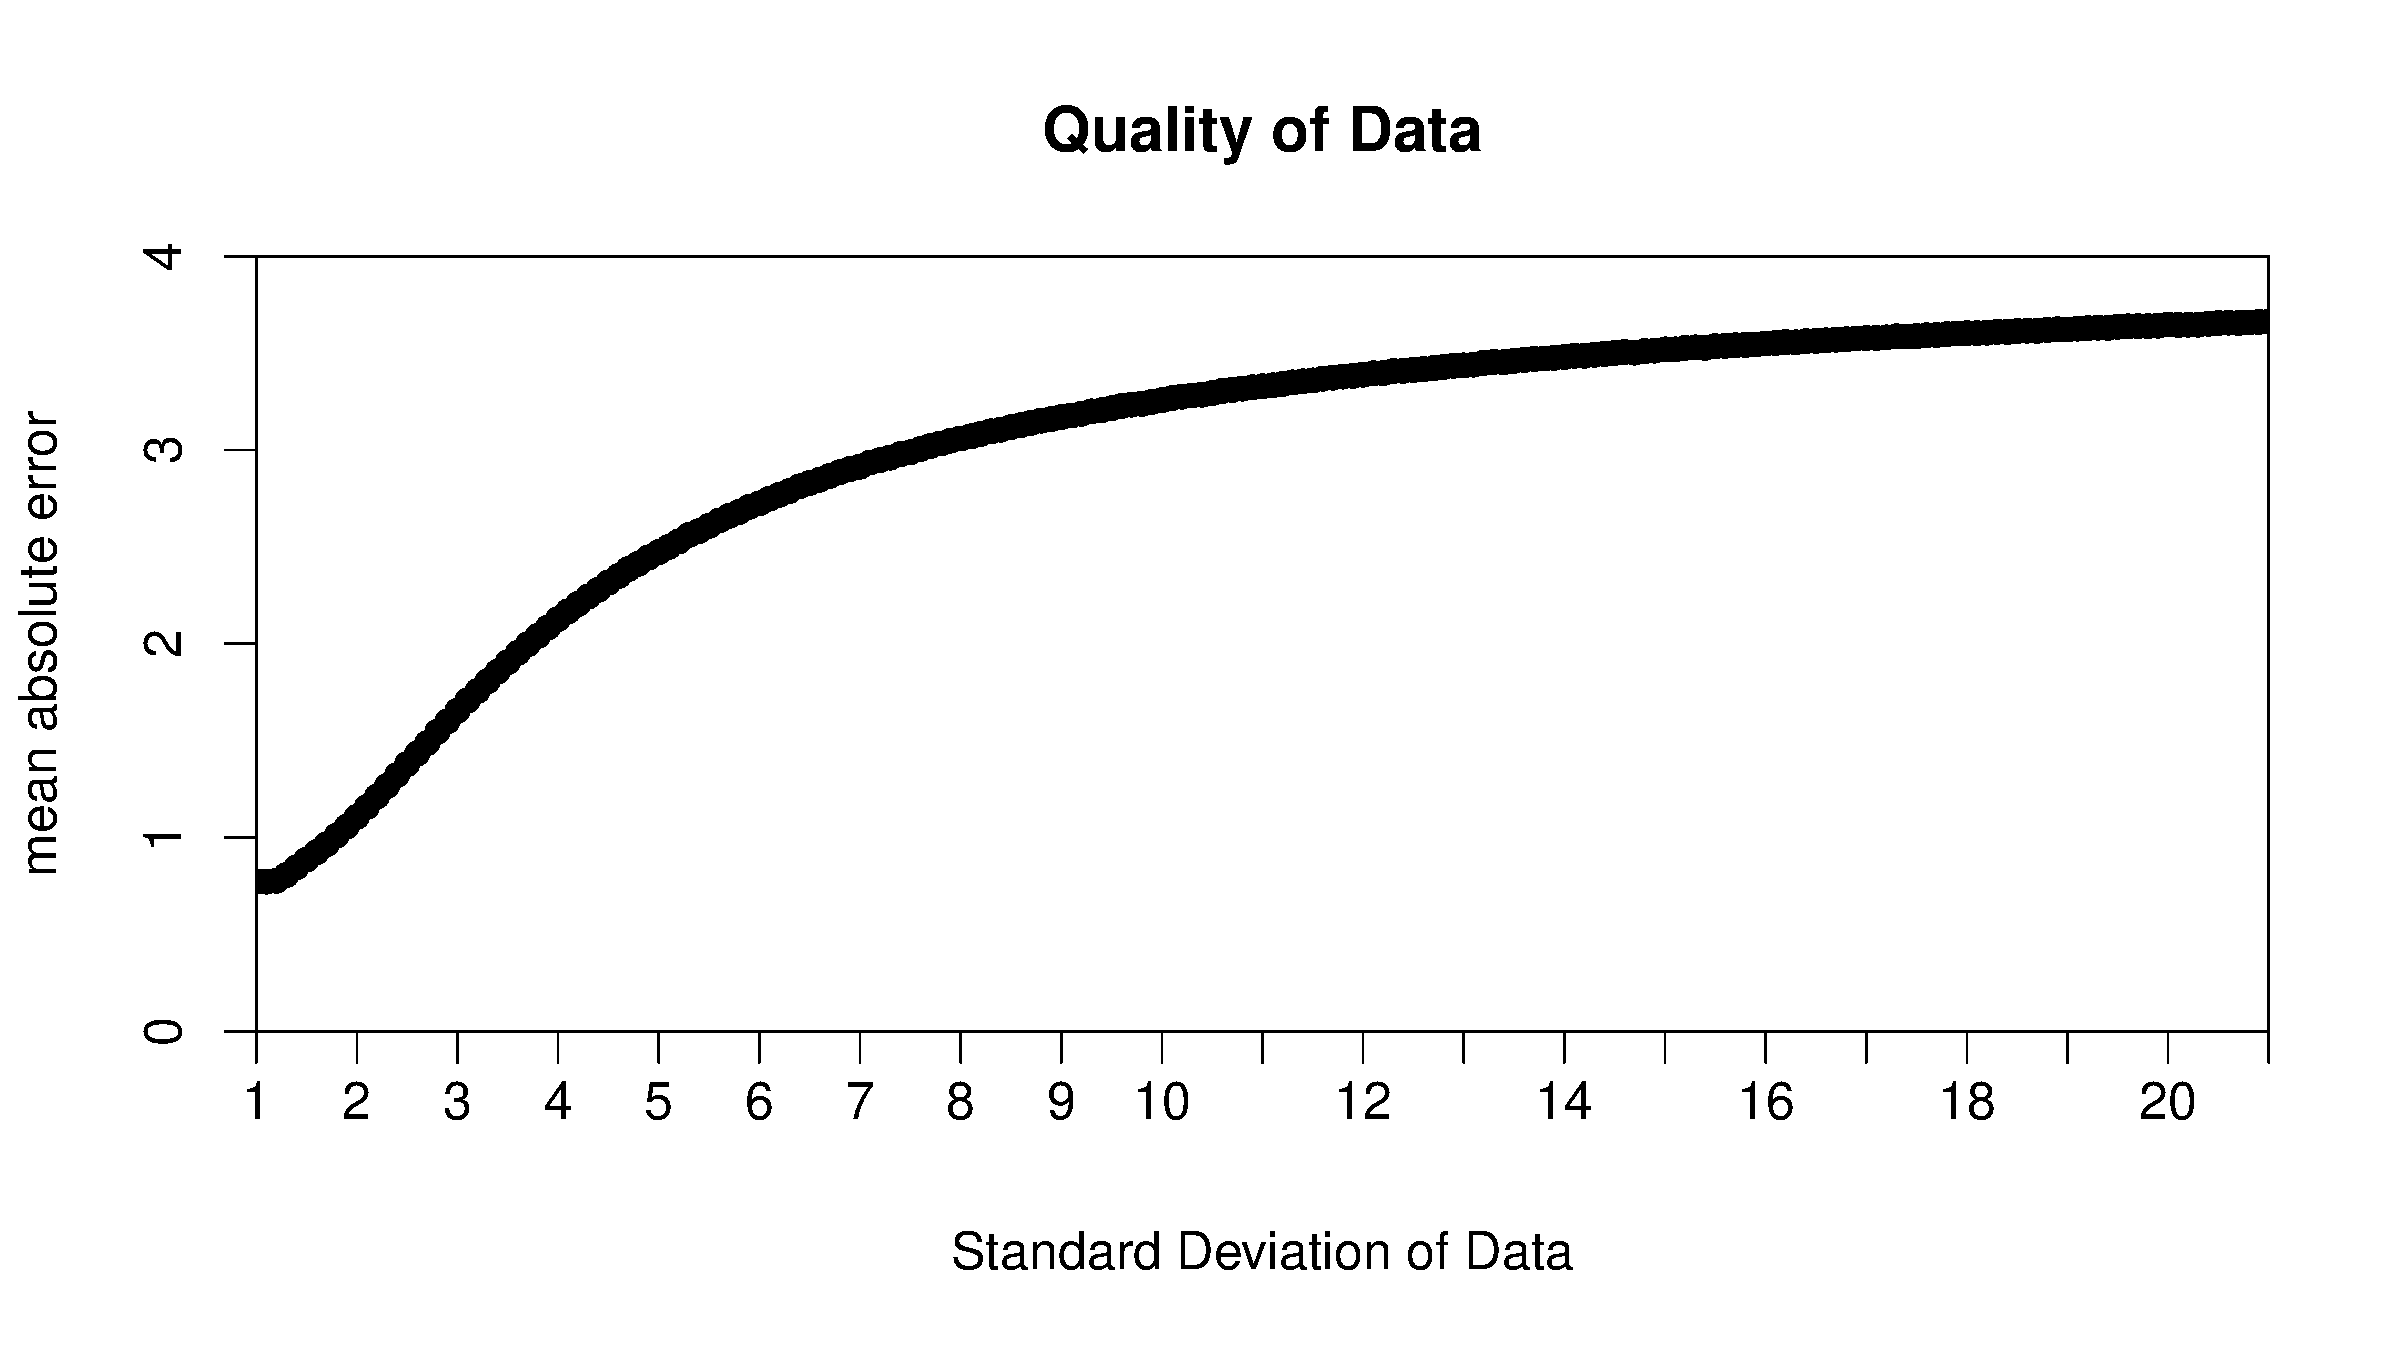
\includegraphics[scale=0.335]{Figures/noise.pdf}
		\rule{35em}{0.5pt}
	\caption[Quality of Data]{Quality of Data}
	\label{fig:noise}
\end{figure}



The mean absolute error increases in a logarithmically fashion with greater noise that is added to the data. This can be explained with the fact that as the noise in the data increases more individual data points take the intensity values of I or IX which are the extremes of the intensity range. This placed an upper limit to the mean absolute error that can be achieved by adding random noise. \\
  
Figure \ref{fig:noiseData} shows the analysis of changing data size and noise level in the data simultaneously. The advantage of more data for the algorithm to learn from seems just relevant for scenarios where there is only a small data set to learn from. Beyond 300 data samples the mean absolute error depends mainly on the level of added noise. This behaviour is exactly what one would expect given that the out-of sample error can be divided into a bias, variance and noise part\citep{LearningFromData}. From the analysis of the influence of data size on the models performance it is known that it suffers from bias. So once enough data samples have been used so that the bias does not change any more the noise level is the only contributing factor.

\begin{figure}[!htpb]
	\centering
		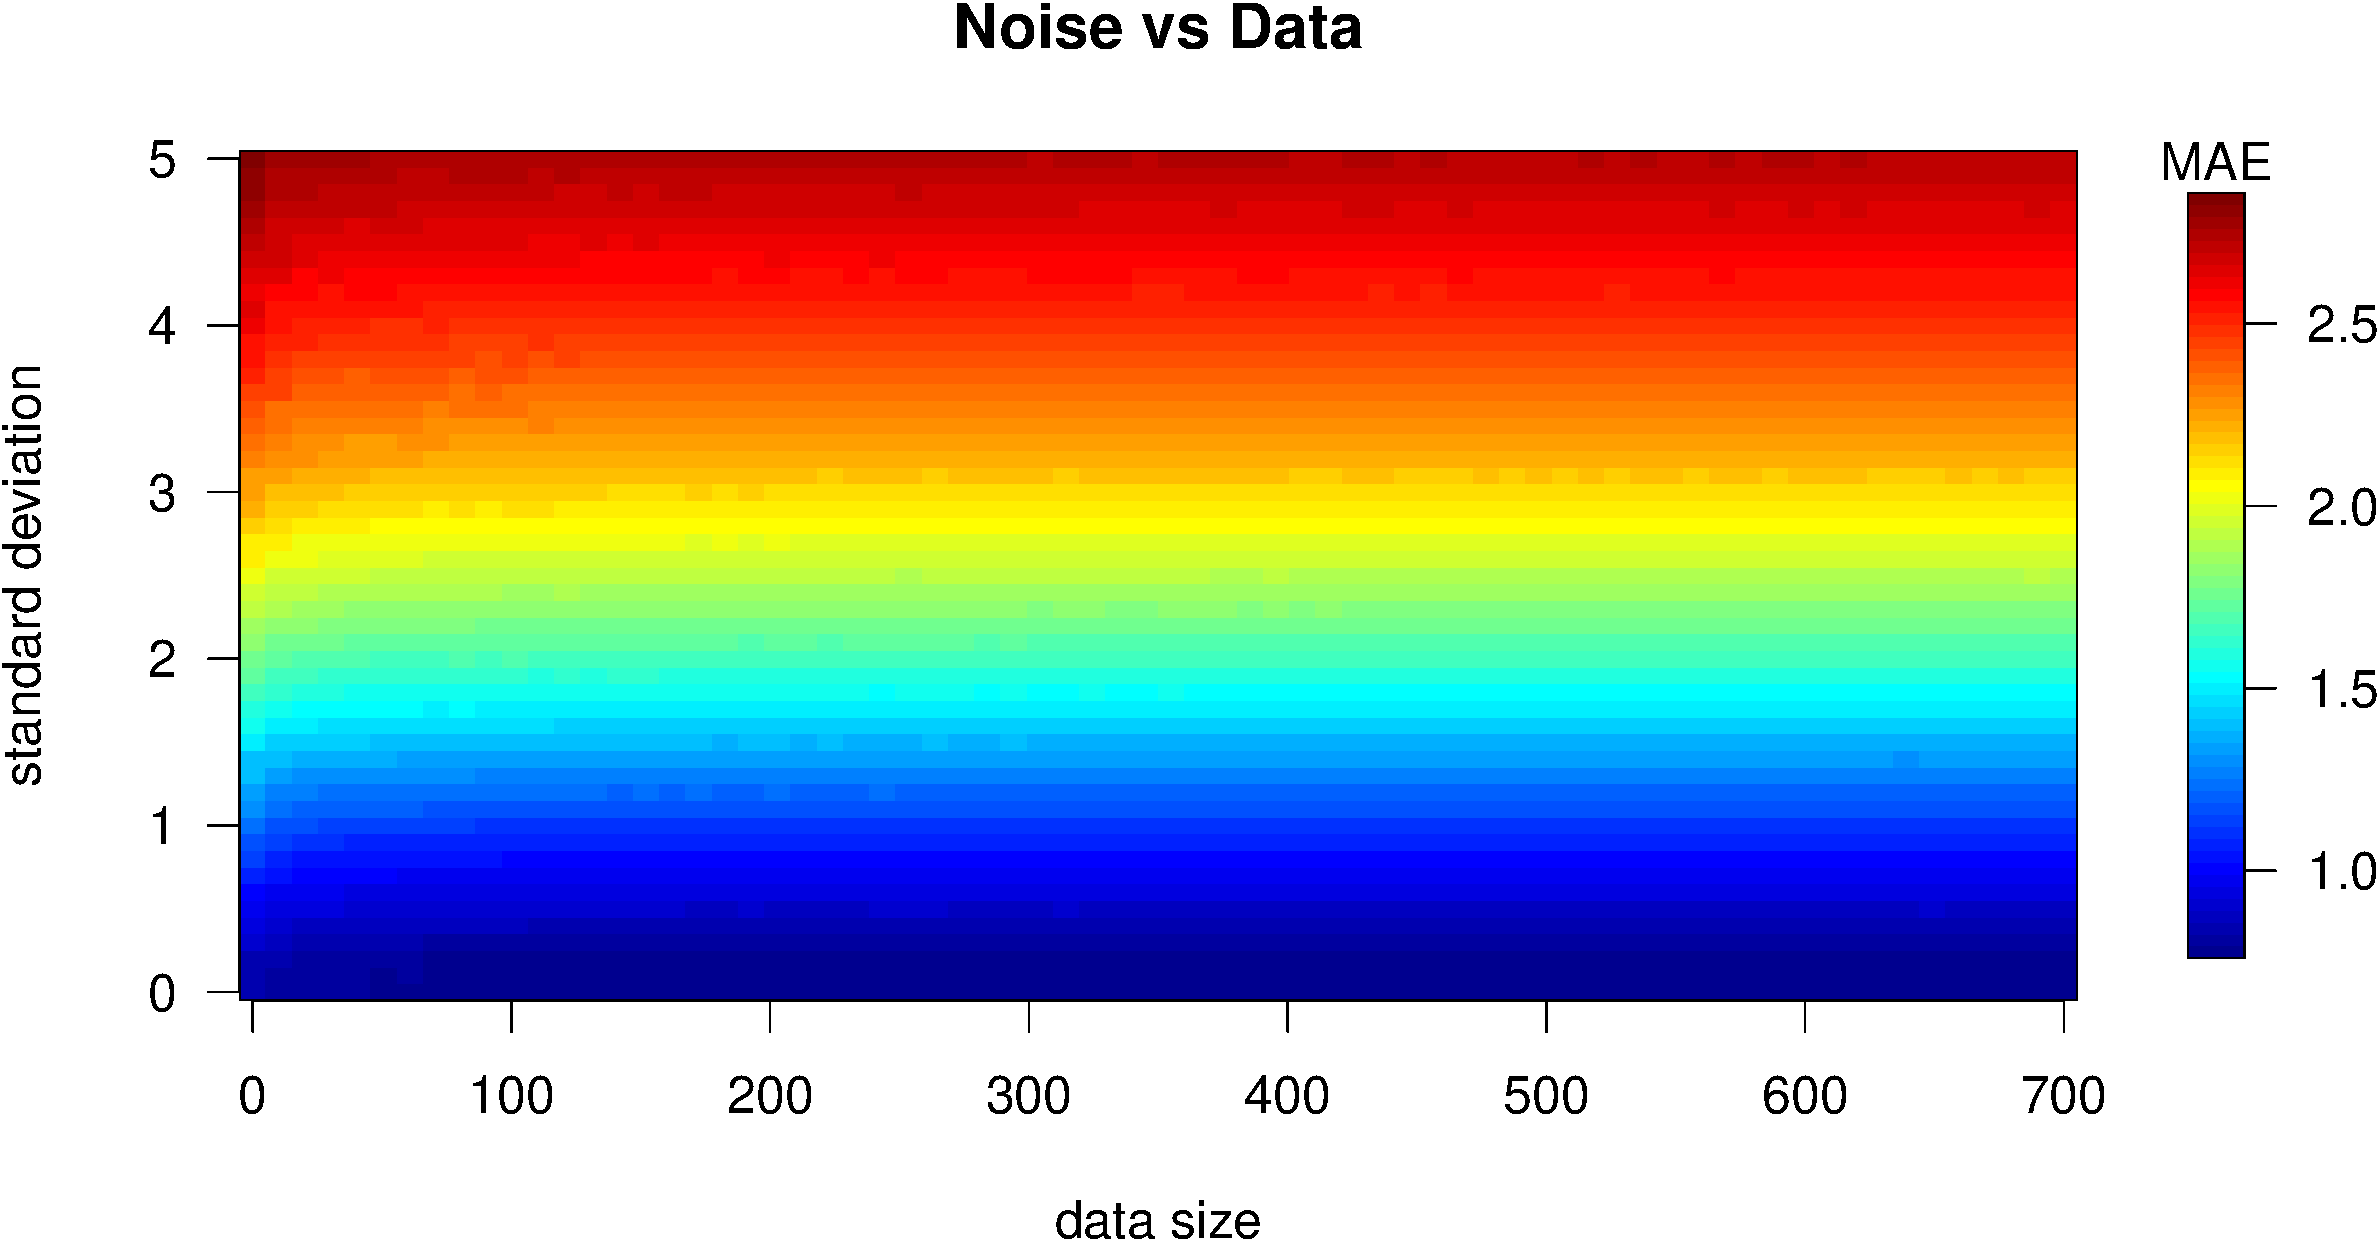
\includegraphics[scale=0.33]{Figures/numberDataNoise.pdf}
		\rule{35em}{0.5pt}
	\caption[Data Size vs Noise]{Data Size vs Noise}
	\label{fig:noiseData}
\end{figure}
\section{Discretization}

One special property of the model by \cite{Rotondi2004} is the discretization of the data into bins of distance. This is necessary since the approach of modelling the intensity distribution by a binomial distribution can only approximate the intensity decay for a certain distance range. To jointly model the intensity distribution an it's dependence on distance one would have to use more advanced techniques like copulas. This subdivision in discrete distance bins is therefore a compromise between enough data per bin to estimate the parameter p of the binomial distribution with great accuracy and enough bins spanning the whole range of site to source distance in order to have a thorough support for the smoothing function. The whole data set of 700 synthetic observations is used and the cross-validation error is chosen as measure of prediction performance. 

\begin{figure}[!htpb]
	\centering
		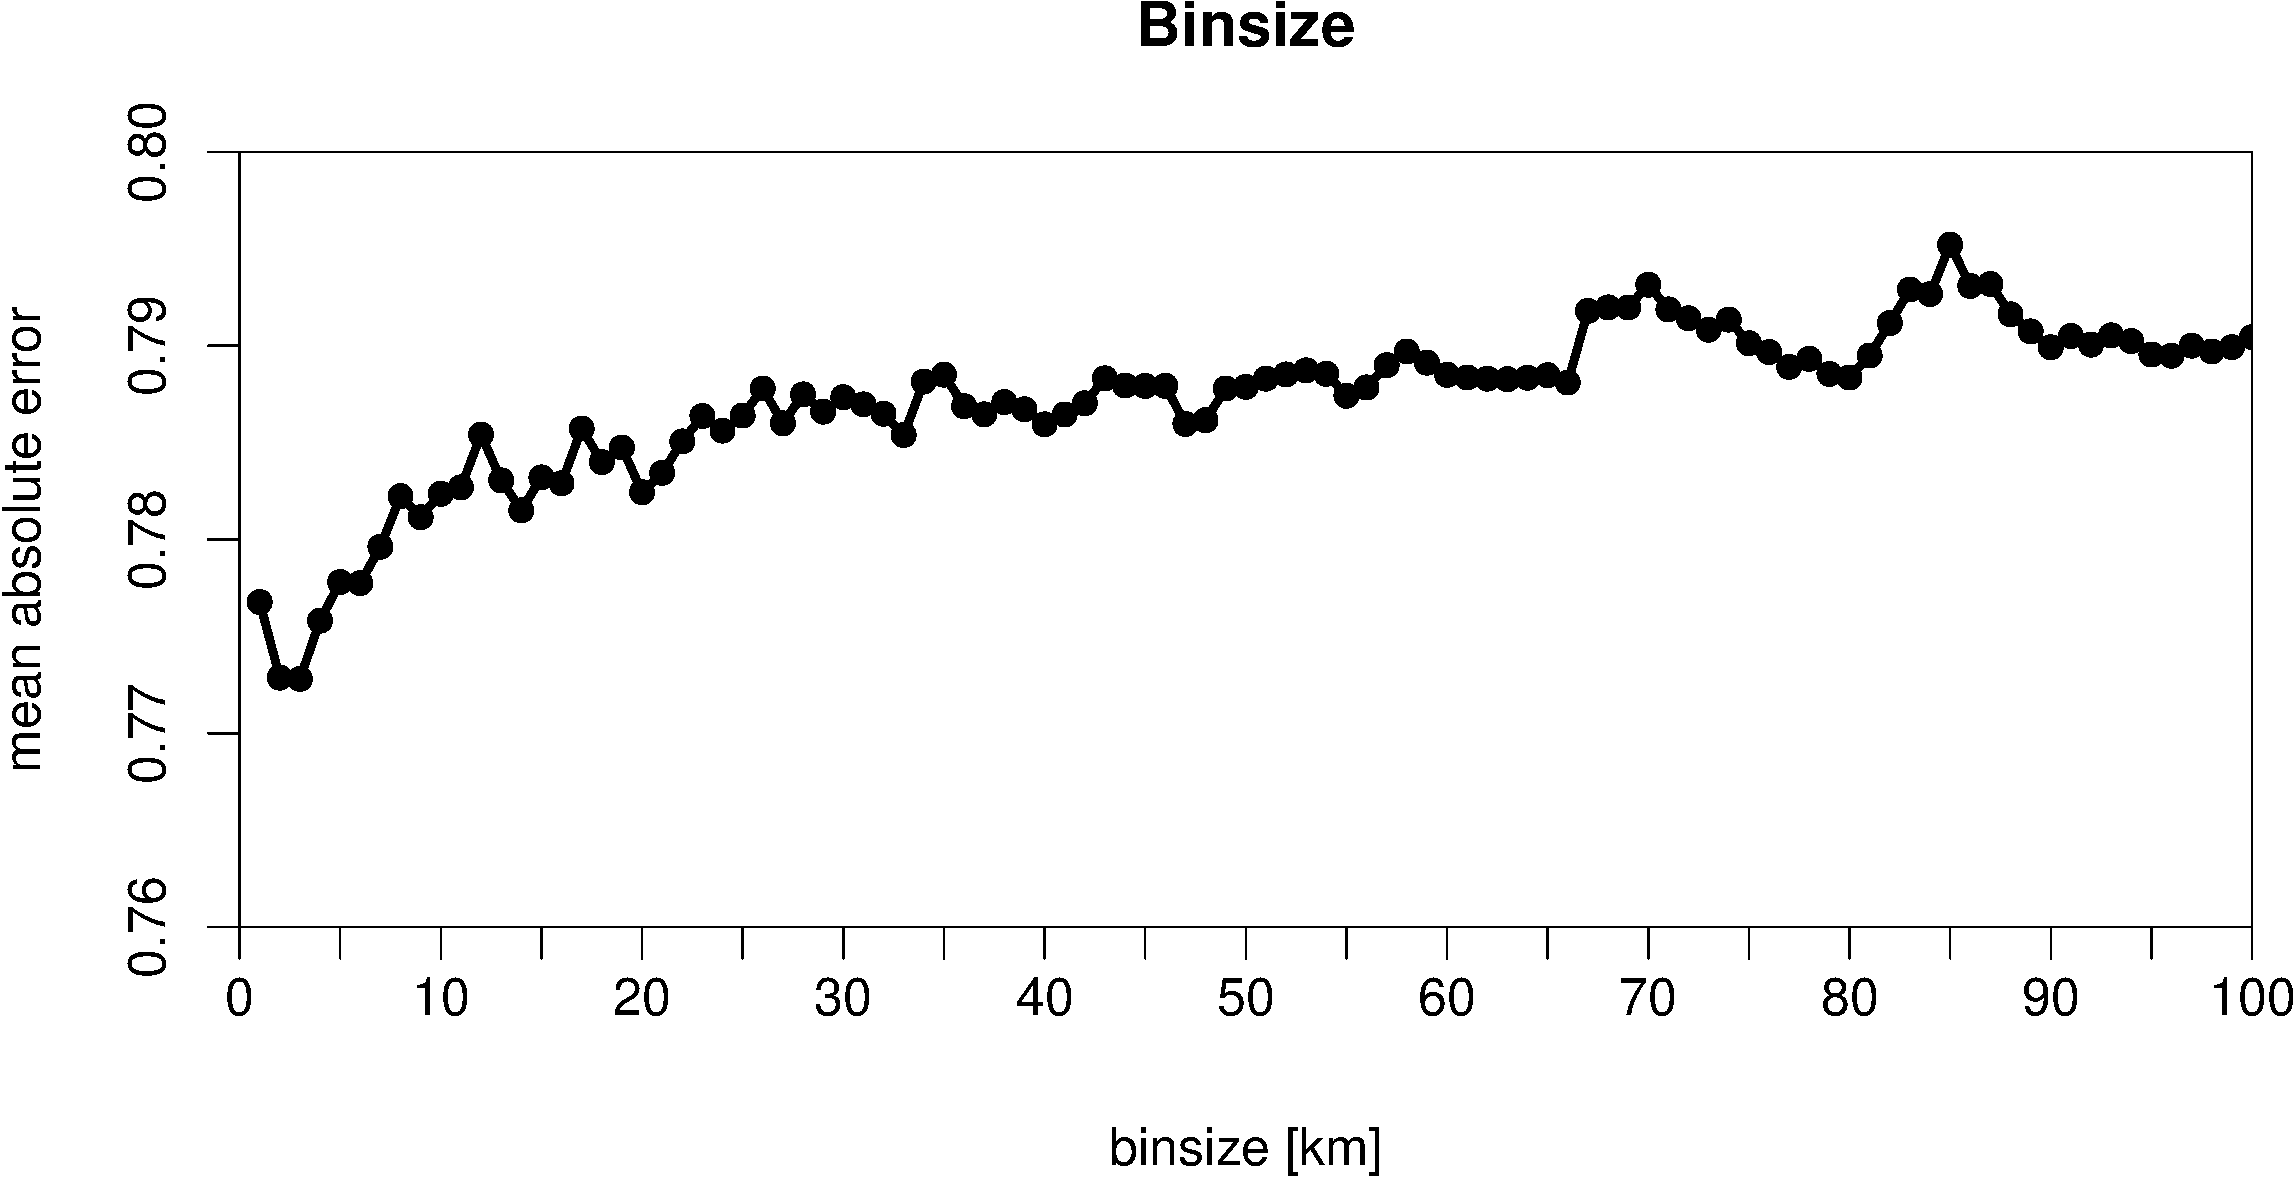
\includegraphics[scale=0.33]{Figures/binsize.pdf}
		\rule{35em}{0.5pt}
	\caption[distance bin size]{distance bin size}
	\label{fig:binsize}
\end{figure}

Figure \ref{fig:binsize} shows the result of a stepwise increase in the width of the distance bins. The lowest mean absolute errors are achieved with bin sizes of 2-3 km. After this point the error increases logarithmically with larger bin widths. It should also be noted that the maximum differences between different bin sizes, and thus the influence of the choice of one particular bin size on the overall error, are relatively small.\\
Figure \ref{fig:binsizeData} shows the results of changing bin size and data size simultaneously. Larger bin sizes affect the mean absolute error on small data sets more heavily than on larger data sets. A general trend of lower errors for smaller bin sizes can be found although this influence is decreased with larger data set size.\\

\begin{figure}[!htpb]
	\centering
		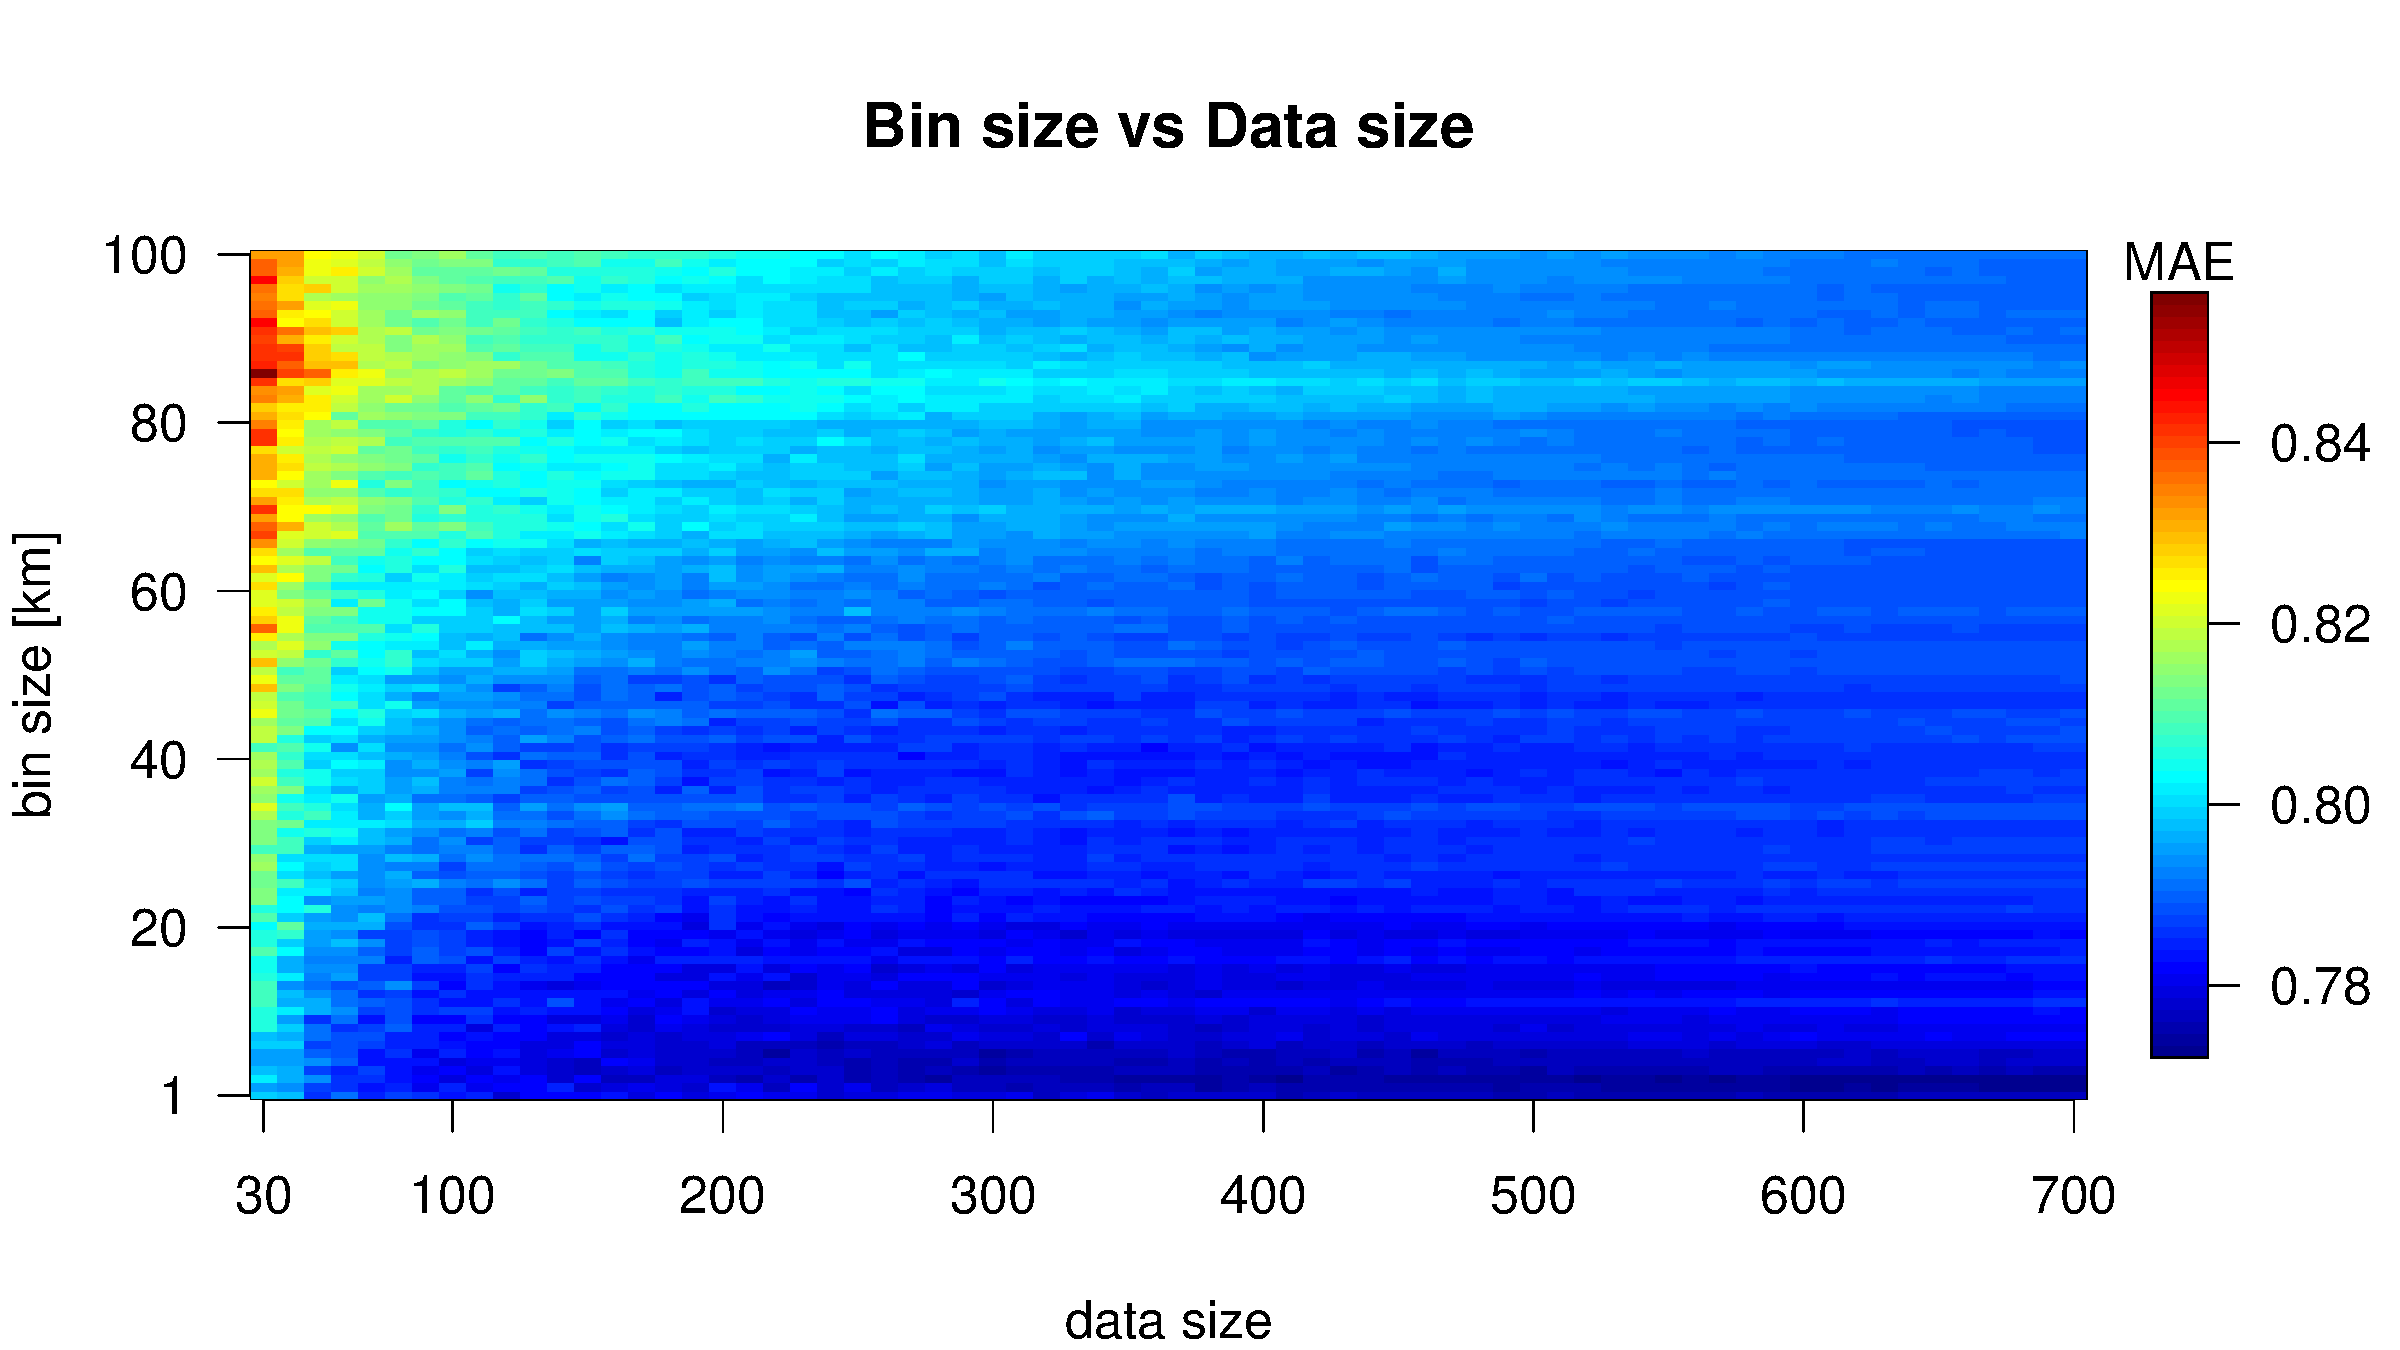
\includegraphics[scale=0.33]{Figures/binsizeDatasize.pdf}
		\rule{35em}{0.5pt}
	\caption[Data Size vs binsize]{Data Size vs binsize}
	\label{fig:binsizeData}
\end{figure}

\section{Sample Bias}
The distribution of samples in distance has up until now be modelled by a uniform distribution. Following the effect of a biased coverage of the distance range on the performance of the model is studied. Therefore, additional to the uniform distance distribution, three distance distributions corresponding to scenarios where the majority of data is available in a middle, a near and a far distance range, respectively, are used to generate synthetic intensity data. The cross-validation error is used as an estimate of the prediction performance.\\
Figure \ref{fig:sampleBias} shows the corresponding distance distributions and the result of this analysis. The lowest mean absolute errors are produced by a uniform distance distribution. The near and middle range distributions differ for a small data size with the near range distribution performing slightly better. But both approach similar error values with larger data sets. The far range distance distribution performs the worst. This is due to the non-linear nature of the intensity decay where most of the information is in the near distance range in which the intensities attenuate more strongly.

\begin{figure}[!htpb]
    \centering
		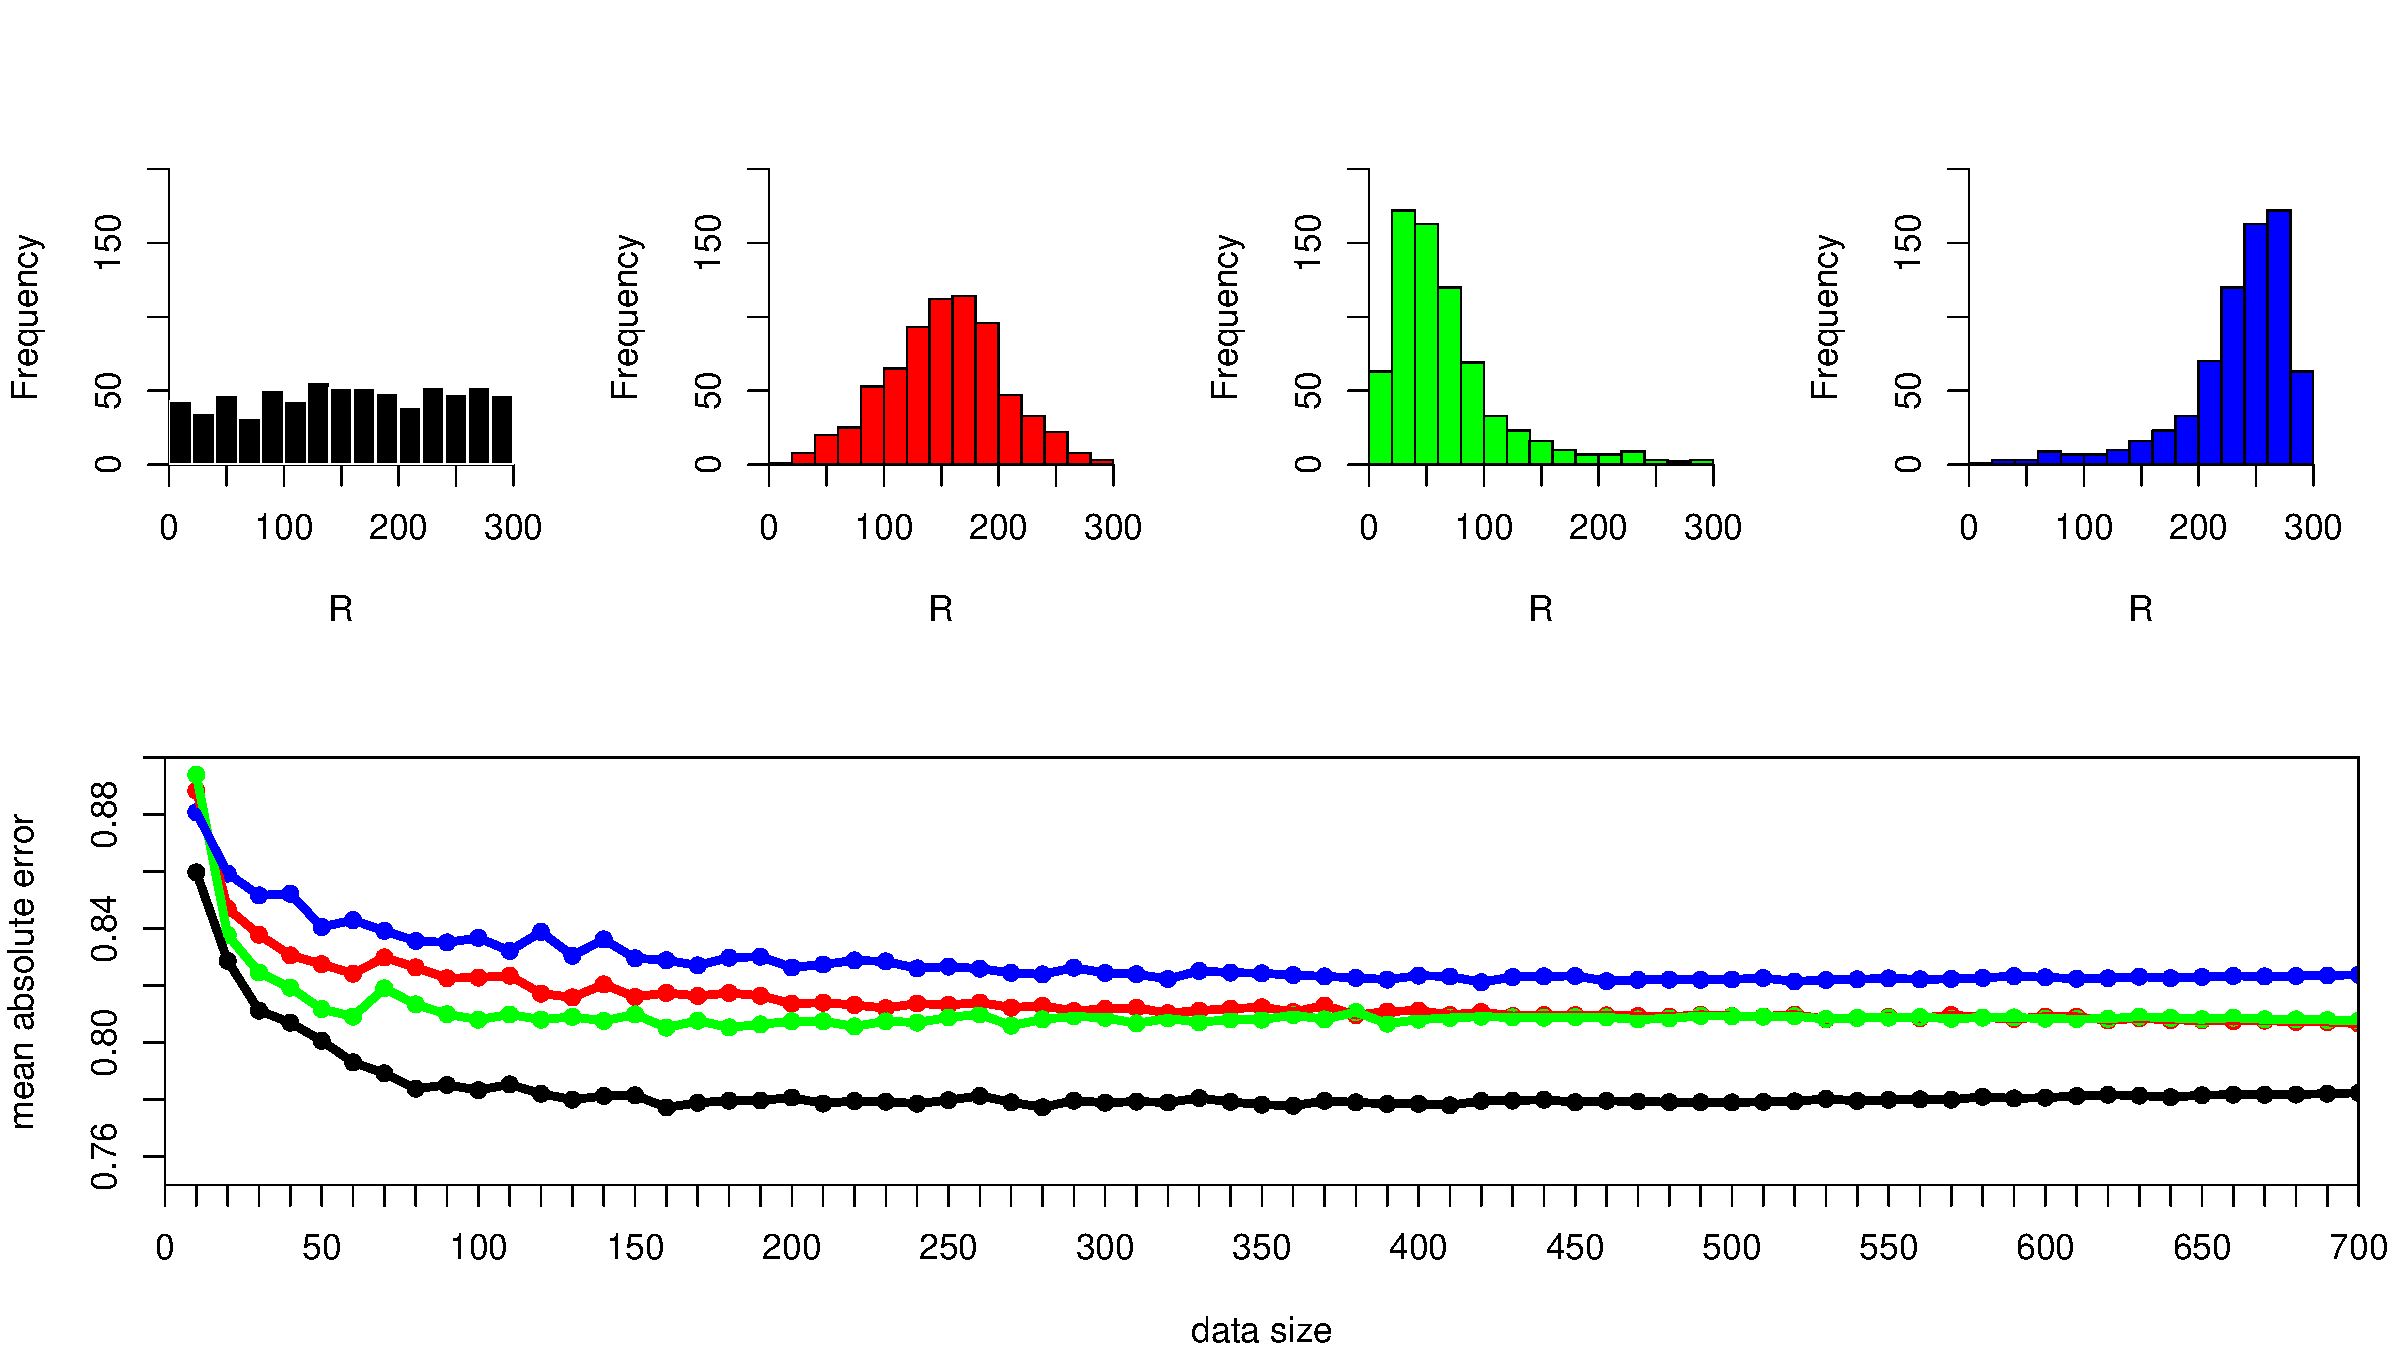
\includegraphics[scale=0.33]{Figures/sampleBias.pdf}
		\rule{35em}{0.5pt}
	\caption[Sample Bias]{Sample Bias}
	\label{fig:sampleBias}
\end{figure}



\section{Choice of Prior Distribution}

A special advantage of a Bayesian approach to ground motion modelling is the possibility to incorporate expert knowledge through the prior distribution. This can be thought of as a start value in a grid-search algorithm where a good start value decreases the number of iterations to find a local and possibly global minimum in the error function. The influence of different prior distribution (table \ref{table:prior}) on the modelling process should be shown. These are a modified version of a prior that \cite{Tsapanos2002} use to compute the hazard for Japanese cities, a uniform distribution, two distributions where the mean decreases linearly and exponentially with distance, respectively, and a distribution that uses the prior knowledge of the already existing IPE by \cite{Koveslighety1906}.\\
The challenge here is that a prior distribution in term of the p parameter and not as intensities given a specific distance is needed. Given that some prior knowledge is available in form of an IPE this can be constructed with the help of the update rules for the hyper parameter $\alpha$ and $\beta$ (Eqn:\ref{eqn:updatehyper}). Since no prior values of $\alpha$ and $\beta$ can be updated these values become zero so that:

\begin{equation}
\alpha = \sum^N_{n= 1} i_s \hspace{2cm} \beta = \sum^N_{n= 1} (I_0 - i_s)
\label{eqn:updatehyperPrior}
\end{equation}

Letting N be equal to 1 this becomes:

\begin{equation}
\alpha = i_s \hspace{2cm} \beta = (I_0 - i_s) = \Delta I
\label{eqn:updatehyperPrior}
\end{equation}

It should be noted that it is not in the scope of this thesis to give a full hands-on tutorial in how to choose a prior distribution for the algorithm of \cite{Rotondi2004}. The aim is to show the influence that a prior can have on the computation. It should also be stressed that a prior distribution in a Bayesian framework acts as a kind of regularization term and it is therefore not advisable to tune the prior distribution so that a minimal error is achieved. A prior should quantify expert or domain knowledge and has to be "naive". \\
Figure \ref{fig:priorMeans} shows the attenuation of the prior distributions' means with increasing distance and three visualizations of the full distribution for distances of 10, 150 and 300 kilometres, respectively. An animation can be found in the electronic supplement: \href{https://github.com/silvioschwarz/master-thesis/tree/master/Masterarbeit/gif/plot.gif}{Animation}.\\
Figure \ref{fig:prior} shows the influence that the different prior distributions have on the mean absolute error with increasing data set size. The difference between the prior distributions is the amount of data it is needed in order for the error to converge to a point where it does not decrease any more. This comes from the fact that the influence of the prior on the learning process is decreased with more data samples. Thus, even a prior that is far of as a starting point of the distribution that is in the data can be overcome by more data samples.

\begin{table}[!htpb]
  \centering
       % \small
       % \setlength\tabcolsep{2pt}
%\setlength\extrarowheight{15pt}
%\def\arraystretch{5pt}
\begin{tabular}{|c|c|c|c|c|}
  \hline
prior & $\alpha$ & $\beta$ & $\mu$ & $\sigma$ \\
\hline 
 \rule{0pt}{7ex}\cite{Tsapanos2002}& $\left(\dfrac{1}{1+\dfrac{R}{60}}\right)^{1/I_0}$ & $1 - \alpha$ & $\dfrac{\alpha}{\alpha +\beta}$ & $\dfrac{\alpha \beta }{(\alpha+\beta)^2(\alpha+\beta+1)}$ \\[5ex]\hline
 \rule{0pt}{7ex}\cite{Koveslighety1906} & $I_s^{Koveslighety}$ & $\Delta I^{Koveslighety}$ &$\dfrac{\alpha}{\alpha +\beta}$ & $\dfrac{\alpha \beta }{(\alpha+\beta)^2(\alpha+\beta+1)}$  \\[5ex]\hline
\rule{0pt}{7ex}Uniform & 1 & 1 & 0.5 & $ 0.08\bar{3}$ \\[5ex]\hline
\rule{0pt}{7ex}Linear & $(\dfrac{1 - \mu}{\sigma} - \dfrac{1}{\mu})* \mu^2$ & $\alpha * \dfrac{1}{\mu -1}$  & $-\dfrac{1}{300}*R $ & $0.007$ \\[5ex]\hline
\rule{0pt}{7ex}Exponential & $(\dfrac{1 - \mu}{\sigma} - \dfrac{1}{\mu})* \mu^2$ & $\alpha * \dfrac{1}{\mu -1}$ & $e^{-0.009*R}$ & $0.007 $ \\[5ex]
   \hline
\end{tabular}
\caption[prior]{prior}
\label{table:prior}
\end{table}


\begin{figure}[!htpb]
    \centering
		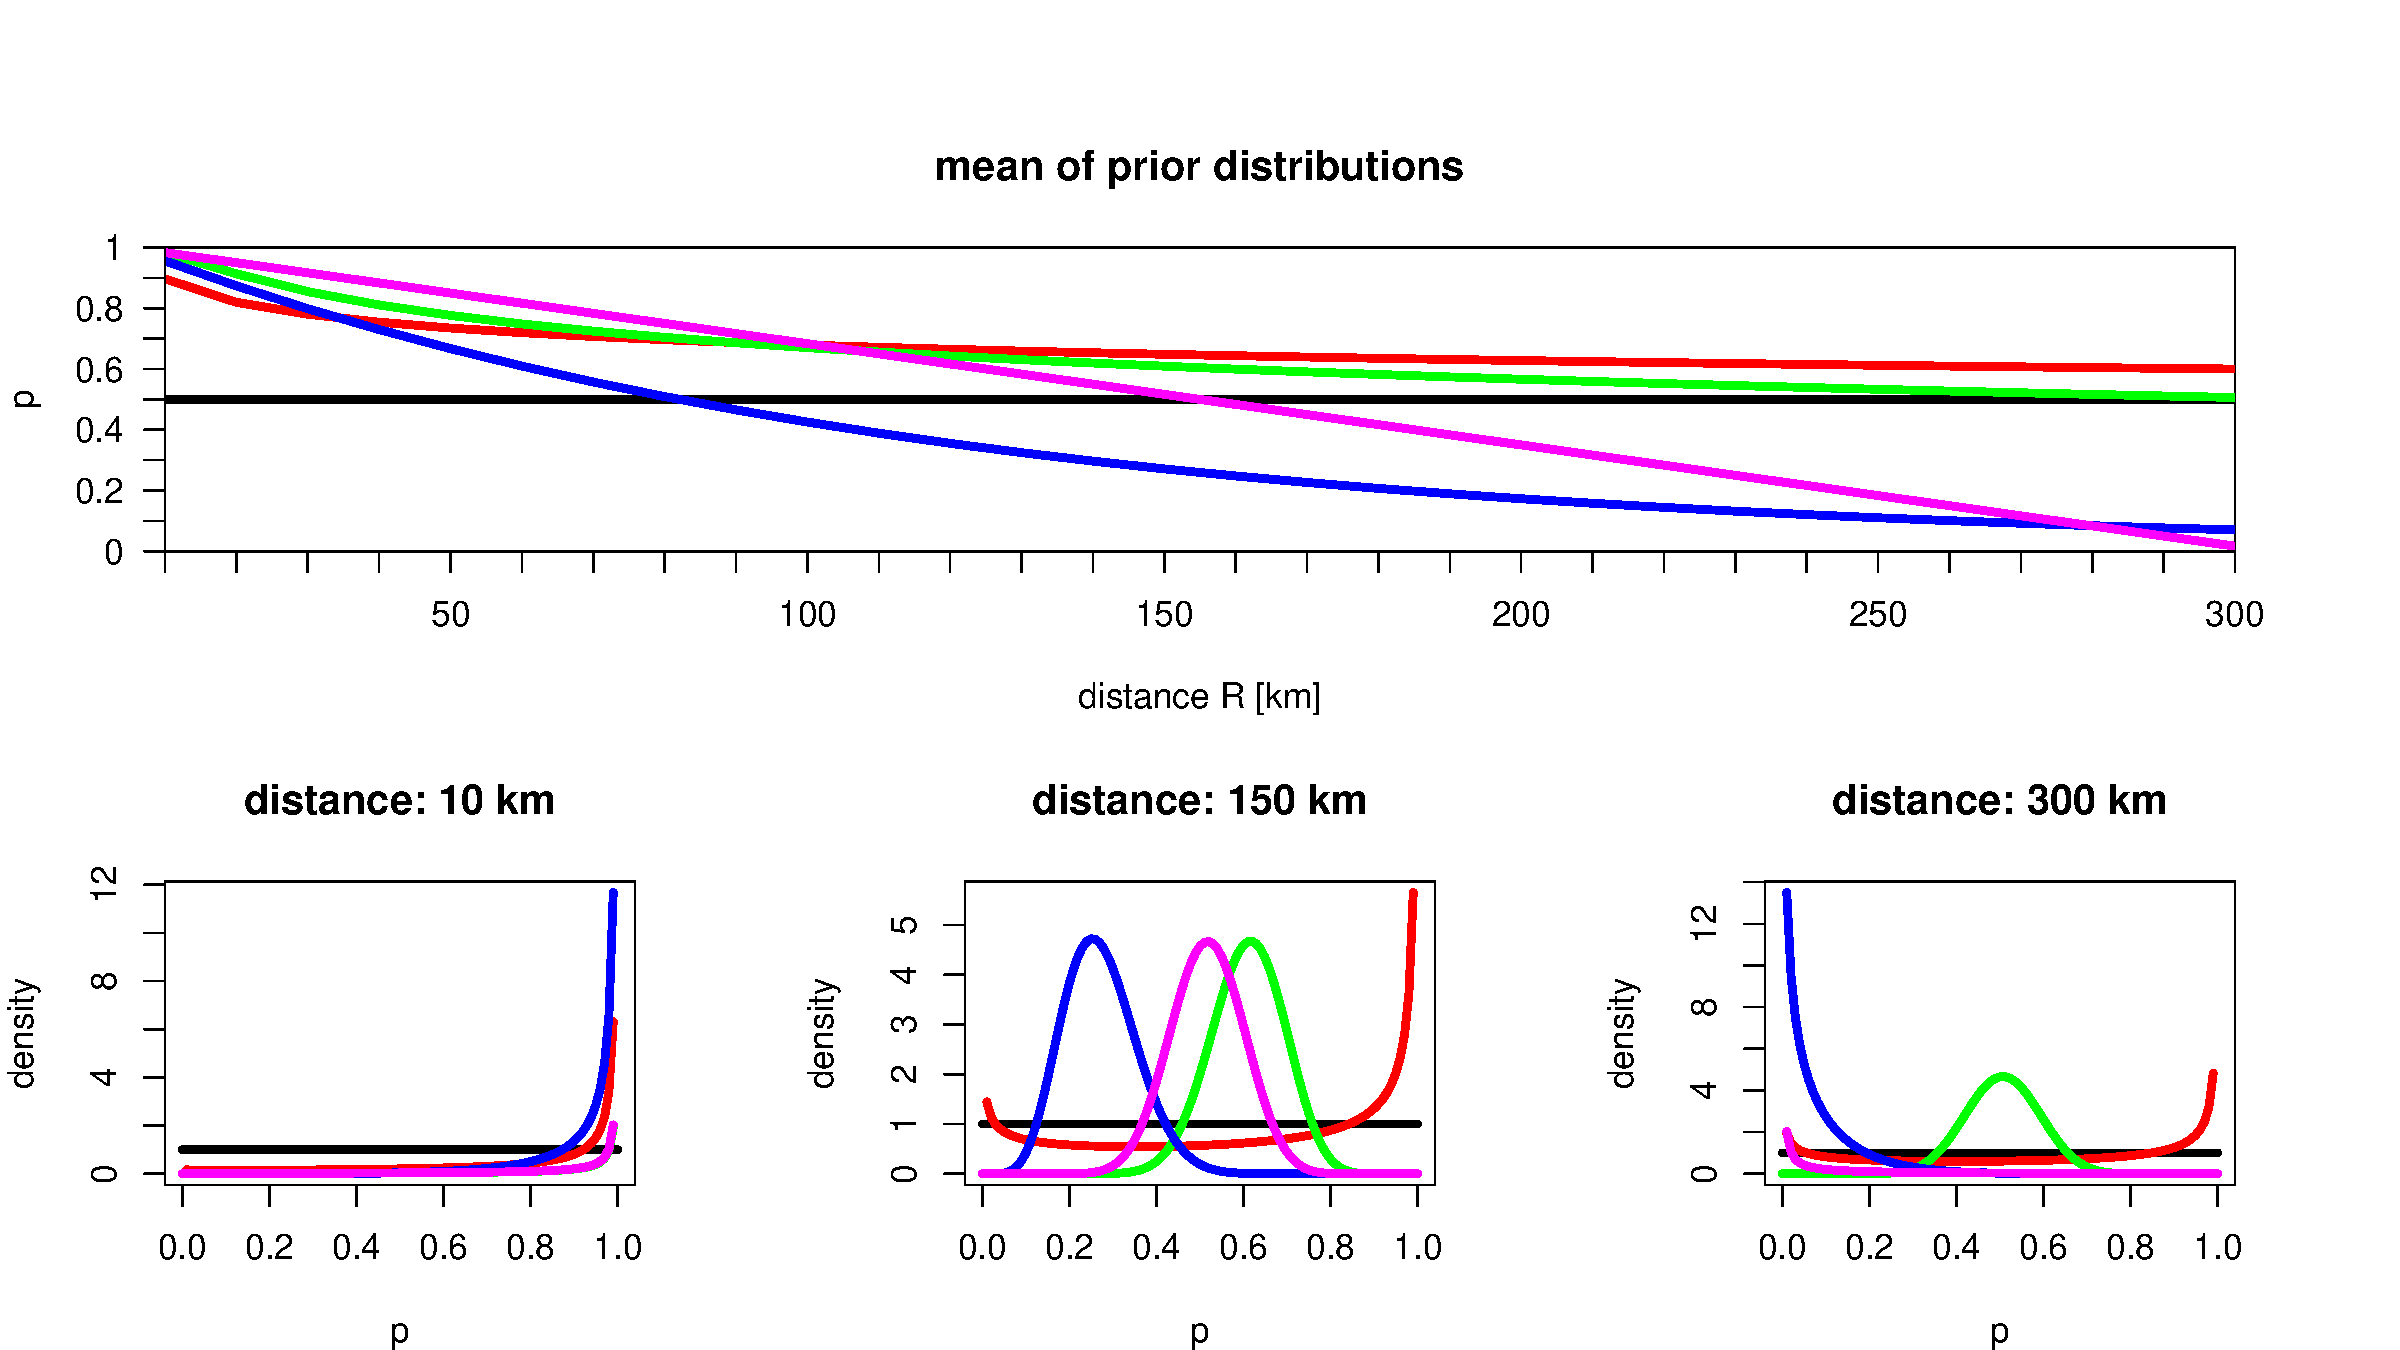
\includegraphics[scale=0.35]{Figures/priorMeans.pdf}
		\rule{35em}{0.5pt}
	\caption[prior]{priorMeans}
	\label{fig:priorMeans}
\end{figure}



\begin{figure}[!htpb]
    \centering
		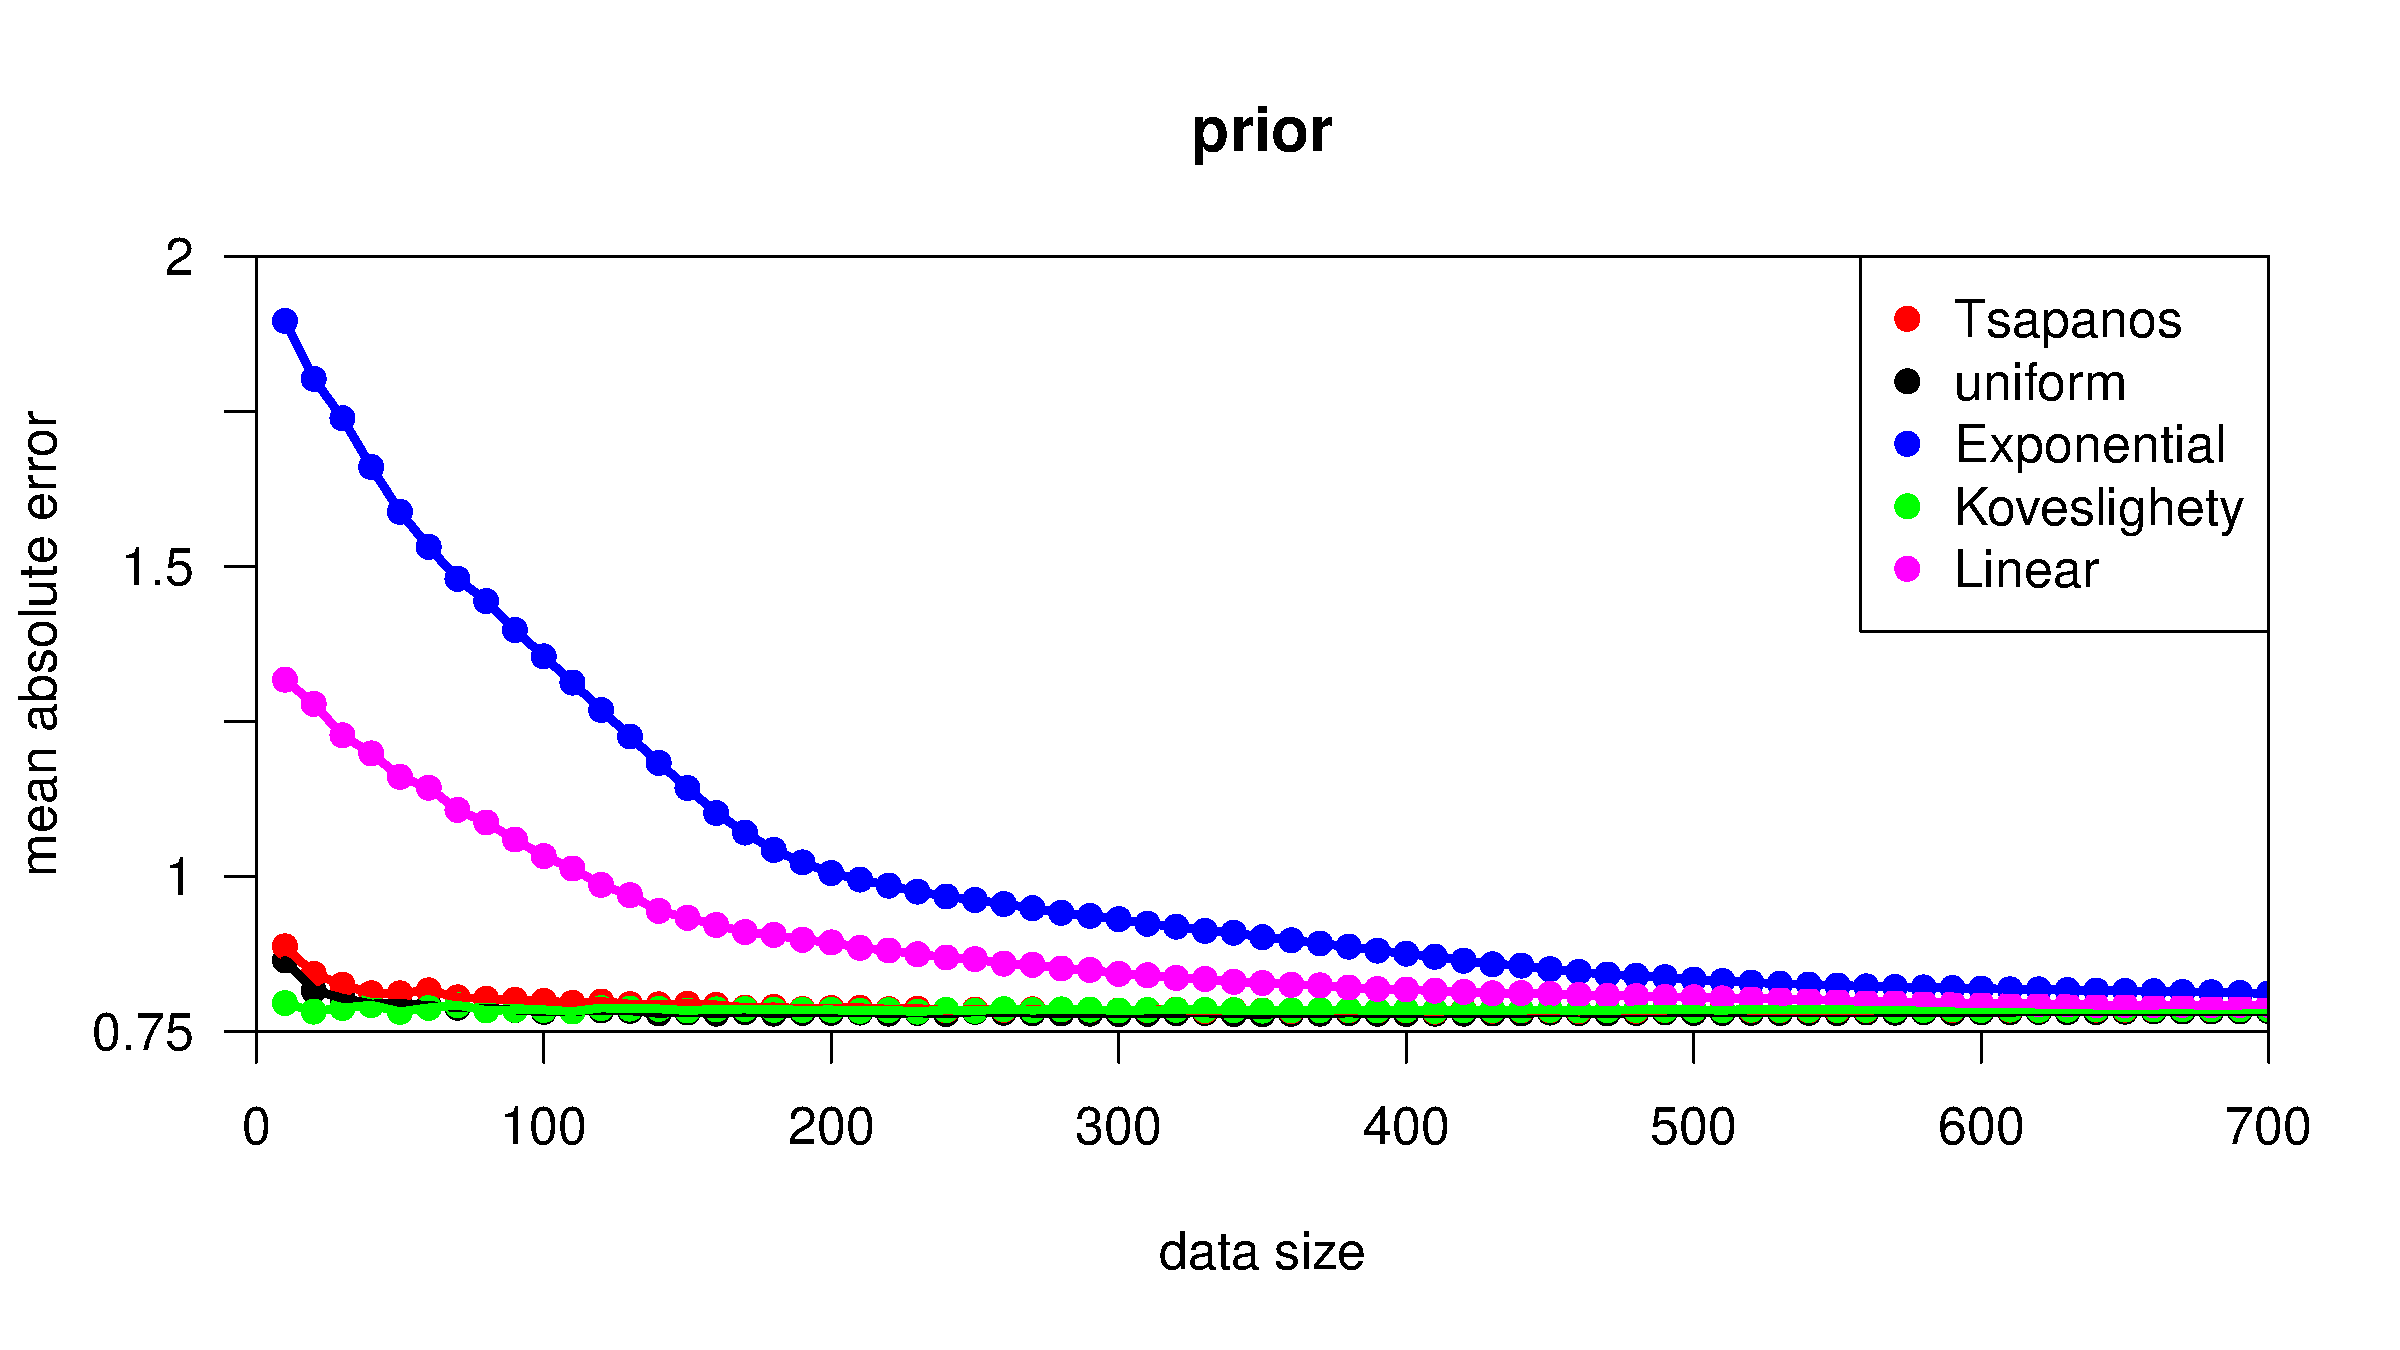
\includegraphics[scale=0.33]{Figures/prior.pdf}
		\rule{35em}{0.5pt}
	\caption[prior]{prior}
	\label{fig:prior}
\end{figure}



\section{Extended Source}


\begin{subequations}
\begin{equation}
\begin{aligned}
&x_1 = x\\ 
& y_1 = y
\end{aligned}
\end{equation}
\begin{equation}
\begin{aligned}
&x_2 = cos(-\theta)*x_1-sin(-\theta)*y_1 \\
&y_2 = sin(-\theta)*x_1+cos(-\theta)*y_1 \\
\end{aligned}
\end{equation}
\begin{equation}
\begin{aligned}
&x_3 = x_2 * \dfrac{b}{a} \\
&y_3 = y_2\\
\end{aligned}
\end{equation}
\begin{equation}
\begin{aligned}
&\gamma = atan(\dfrac{y_3}{x_3} )-atan(\dfrac{y_2}{x_2} )+abs(\theta)\\
&x_4 = cos(\gamma)*x_3-sin(\gamma)*y_3\\
&y_4 = sin(\gamma)*x_3+cos(\gamma)*y_3
\end{aligned}
\end{equation}
\label{eqn:transformR}
\end{subequations}

\begin{figure}[!htpb]
    \centering
		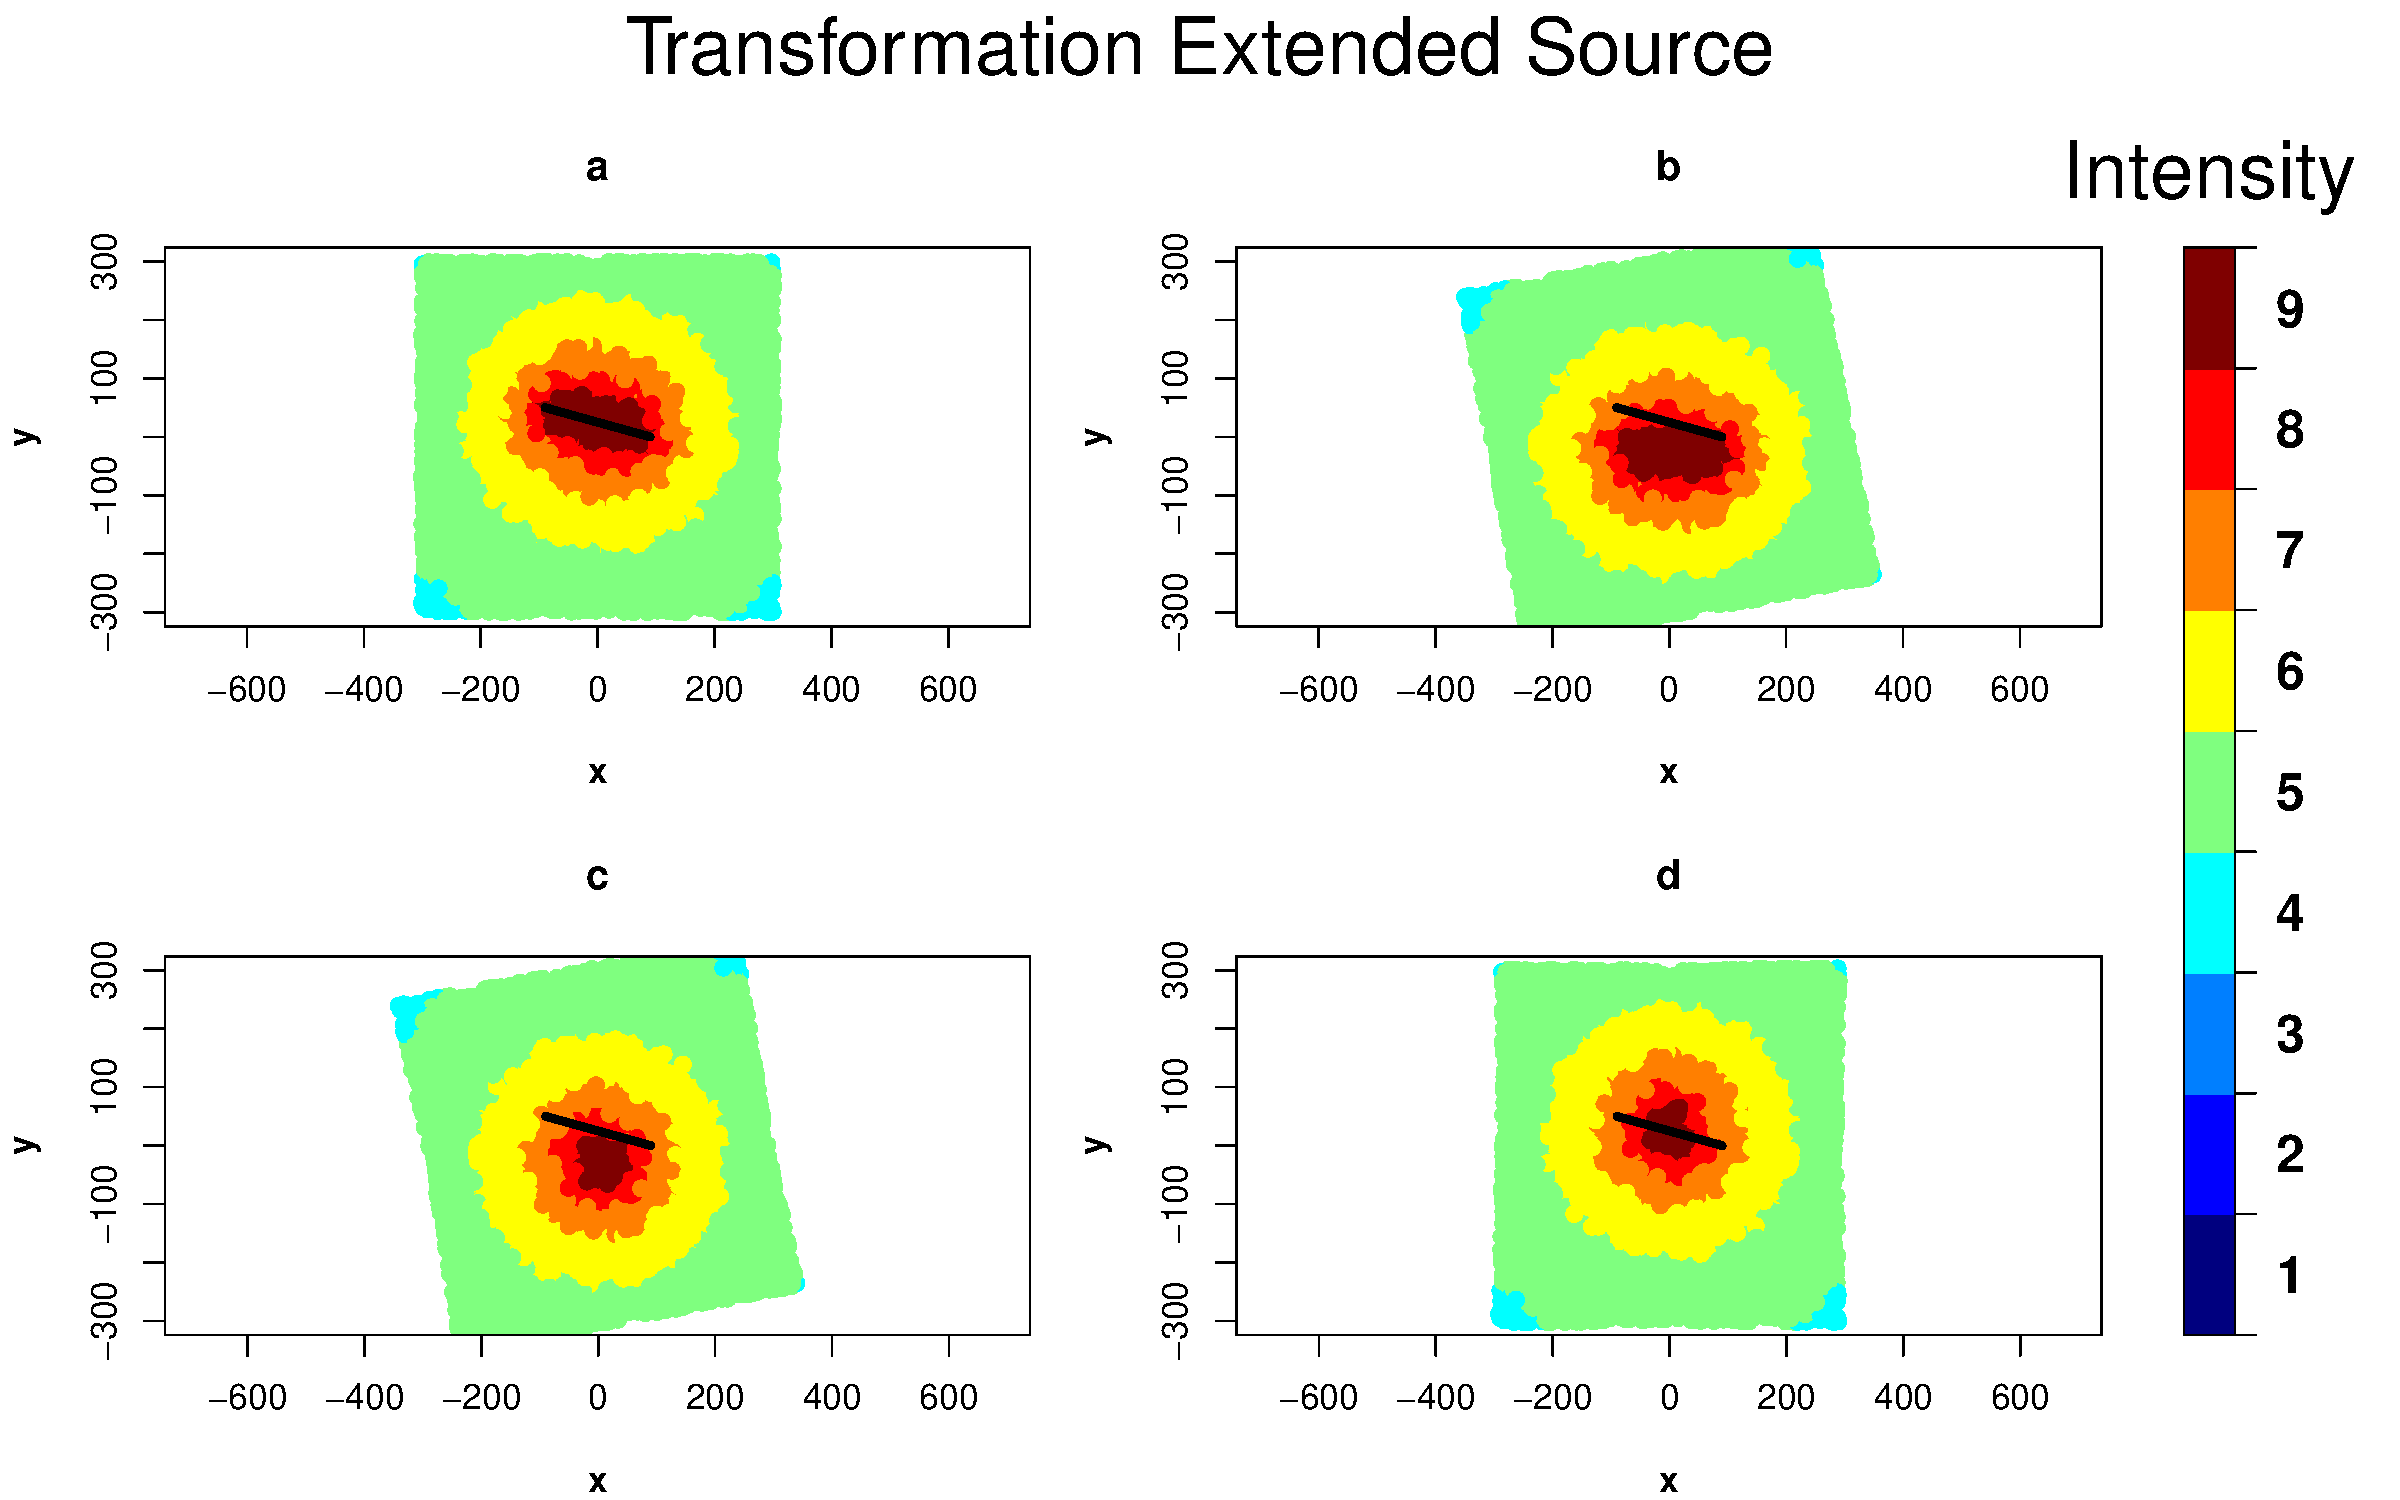
\includegraphics[scale=0.35]{Figures/extendedSource.pdf}
		\rule{35em}{0.5pt}
	\caption[extended Source]{extended Source}
	\label{fig:extendedSource}
\end{figure}

Results: 0.1551224 0.2623517 